%chapter 4
%Pole Stability and Obliquity Evolution under Boulder-Induced YORP Torques
\chapter{Obliquity Evolution under Boulder-Induced YORP Torques}
\label{yorp_obliquity}

%\section{Background} \label{background} %section 1
%asteroids
%Asteroids are highly variable bodies that retain the history of our solar system in their motion, geology, and mineral composition. The dynamics of asteroids can be highly sensitive in the sub-1 km diameter regime. At this size range, we often find rubble-piles formed by the aggregation of material leftover from a previous impact. These types of asteroids can experience multiple forms as they transition in their dynamics and are accelerated to either high velocity disaggregation or low velocity chaotic tumbling \citep{Golubov2019}. 
%Here we investigate the unique thermal properties seen and modeled by the Yarkovsky-O'Keefe-Radzievskii-Paddack (YORP) effect, which is an additional force due to photons re-radiating from the surface as governed by the material thermal inertia and thermal skin depth \citep{Rubincam2000}\citep{Davidsson2014}. This is opposite to the solar radiation pressure experienced by small bodies, which is the force of incident radiation. This YORP force has been known to shift the spin and pole directions of bodies over time and has been observed in the accelerations of multiple bodies from the ground \citep{Durech2023}\citep{Lowry2007}. 

%Analytical models of the YORP effect can take a shape-focused approach with relaxed thermal assumptions, while others have developed detailed thermal models while assuming general properties of the shape \citep{Scheeres2007}\citep{Nesvorny2008}. The latter is useful when applying the YORP theory to many bodies constrained by ground observations. In this work, we will further extend Scheeres' geometric analysis of YORP torque to include the possibility of boulders which will be an additive measure for estimates taken from the ground where detailed features are not seen. In geometric simulations, we have simulated and verified that YORP is extremely sensitive to small changes in the shape, which means that a mismodeled boulder may alter YORP estimates up to 200\% \citep{Baker2024} \citep{Statler2009}. 

%Boulders on asteroid surfaces experience the intra-radiative effect called tangential YORP, where at optimal spin velocities and thermal inertias, boulders will absorb and then transmit thermal energy in the pro-spin direction \citep{Golubov2022}. It is also seen that obliquity is a large driver of varying the magnitude of tangential YORP \citep{Sevecek2016}. It is suggested that the presence of unmodeled tangential YORP is the reason for the disagreement in the YORP acceleration calculated and measured for the asteroid Itokawa (cite Golubov again). There are also YORP torques induced by crater shapes. This is unique from normal YORP as it considers self-heating and self-shadowing effects that are activated by the concavity \citep{Zhou2023}.

%Our model will give the YORP torque due to the heat absorbed to the thermal depth of boulders and compare the relative strength of added torque between the normal and tangential YORP effects. This is not a new theory for thermal behavior or YORP interaction. It is an extension of previous efforts made to constrain stochasticity in YORP by modeling small details \citep{Statler2009} \citep{Rozitis2012}. We apply geometric models of faceted shapes with different thermal assumptions. Many boulders are simulated in order to capture a full test of significance of features that vary in location, orientation, and size. There is further analysis to be done with different shapes and asymmetries. More boulders could be added as well as the regolith roughness, similar to the thermal beaming effect \citep{Rozitis2011a}.  

%give more info on chaotic tumbling boulders?

We continue to model the sizes, positions, and orientations of boulders and randomize these properties to characterize the upper and lower bounds to YORP variability. In studying the shifting obliquity angle rate, we are also analyzing the ease of inducing instability in the dynamics. While the spin acceleration can be derived from longitudinal asymmetry and surface area, the angle acceleration depends on full 3-D asymmetry and the thermal inertia which governs where in the spin period the torque due to YORP is applied. The goal of investigating variance in the obliquity rate induced by the YORP effect originating from surface boulders is to find how much more likely a rough shape is to reach a YORP end-state. In this approach, we will not consider surface redistribution, however this is to be expected when varying the dynamics of a body. For this purpose, it is assumed that surfaces stay static until they reach their spun-up or spun-down dynamical end-state.  

%My question here is, how much asymmetry from boulders is required to induce rapid spin-up or down in an asteroid? I can use the total western surface area as a variable. I will analyze the total size/mass contribution. I can show the reduction in YORP timescale. I will also do a time propagation of these EOMs to show interplay between angular velocity and angle rate change. I can simulate the removal of different boulders at different time steps as the body spins up.  

%pole instability
%thermal properties
%YORP modeling
%The paper is organized as follows. We begin by describing the important frames of reference for our force model in Section \ref{coord}. Next we review the equations for YORP torque by summed facets in Section \ref{yorp}, and then describe the methods we apply to examine the spin and stability dynamics induced by boulders in Section \ref{spin}. After this description of the methods, we will present the results in Section \ref{results}, and finally the discussion and conclusion will be in Sections \ref{discussion} and \ref{conclusion}, respectively. 


% \section{Coordinate Frames}\label{coord}

% The coordinate frames required to examine YORP obliquity evolution are the inertial frame, the body-fixed frame, and the heliocentric orbit frame. The variables of motion being used are expressed in the body and orbital contexts. The inertial frame is given by the unit vectors $\mathbf{\hat{X}}_i, \mathbf{\hat{Y}}_i,$ and $\mathbf{\hat{Z}}_i$. The heliocentric orbit frame is then defined by $\mathbf{\hat{X}}_H$, which is the unit vector pointing towards the argument of perihelion, $\mathbf{\hat{Z}}_H$, which aligns with the orbit angular momentum direction out of plane, and $\mathbf{\hat{Y}}_H$, the third vector which completes this right-handed frame definition and aligns with the velocity vector at perihelion passage.
% Applying classical orbit elements, we express our heliocentric orbit frame in the inertial frame as follows.
% \begin{equation}
% \begin{split}
% \mathbf{\hat{X}}_H = &[cos \: \bar{\omega} \:cos\:\Omega - sin \:\bar{\omega}\:sin\:\Omega cos \:i] \mathbf{\hat{X}}_E \\
% & + [cos\:\bar{\omega}\:sin\:\Omega + sin\:\bar{\omega}\:cos\:\Omega \:cos\: i] \mathbf{\hat{Y}}_E \\
% & + sin\: \bar{\omega} \:sin \:i \mathbf{\hat{Z}}_E
% \end{split}
% \end{equation}
% \begin{equation}
% \begin{split}
% \mathbf{\hat{Y}}_H = &-[sin \: \bar{\omega} \:cos\:\Omega + cos \:\bar{\omega}\:sin\:\Omega cos \:i] \mathbf{\hat{X}}_E \\
% & + [-sin\:\bar{\omega}\:cos\:\Omega + cos\:\bar{\omega}\:cos\:\Omega \:cos\: i] \mathbf{\hat{Y}}_E \\
% & + cos\: \bar{\omega} \:sin \:i \mathbf{\hat{Z}}_E
% \end{split}
% \end{equation}
% \begin{equation}
% \begin{split}
% \mathbf{\hat{Z}}_H = sin \: \Omega \: sin\: i \mathbf{\hat{X}}_E - cos \: \Omega\: sin i \mathbf{\hat{Y}}_E + cos i \:\mathbf{\hat{Z}}_E
% \end{split}
% \end{equation}
% In these equations, $i$ is inclination of the orbit, $\Omega$ is the longitude of ascending node, and $\bar{\omega}$ is the longitude of ascending node as per Scheeres' 2007 notation. We will make use of the body frame notation in our equations of motion in order to describe the YORP accelerations experienced by the surface and how they are influencing the spin pole directly. These forces can be translated to the orbital or inertial frame by these frame definitions given here. The body frame is defined here with variable definitions to follow.

% \begin{equation}
%     \begin{split}
%     \mathbf{\hat{x}}_B = &[sin \: \alpha \: cos \: \phi \: + \: cos \: \alpha \: sin \: \phi \: sin \: \delta]\mathbf{\hat{X}}_E \\
%     + &[cos \: \alpha \: cos \: \phi \: - \: sin \: \alpha \: sin \: \phi \: sin \: \delta]\mathbf{\hat{Y}}_E \\
%     + &sin \: \phi \: cos \: \delta \mathbf{\hat{Z}}_E
%     \end{split}
% \end{equation}
% \begin{equation}
%     \begin{split}
%     \mathbf{\hat{y}}_B = &[sin \: \alpha \: sin \: \phi \: + \: cos \: \alpha \: cos \: \phi \: sin \: \delta]\mathbf{\hat{X}}_E \\
%     - &[cos \: \alpha \: sin \: \phi \: + \: sin \: \alpha \: cos \: \phi \: sin \: \delta]\mathbf{\hat{Y}}_E \\
%     + &cos \: \phi \: cos \: \delta \mathbf{\hat{Z}}_E
%     \end{split}
% \end{equation}
% \begin{equation}
%     \begin{split}
%     \mathbf{\hat{z}}_B = &cos \: \alpha \: cos\: \delta\mathbf{\hat{X}}_E \:+ \: sin \: \alpha \: cos \: \delta\mathbf{\hat{Y}}_E  + \: sin \: \delta \mathbf{\hat{Z}}_E
%     \end{split}
% \end{equation}
% In these unit vector definitions, $\alpha$ is the right ascension of the asteroid spin pole, $\delta$ is the declination, and $\phi$ is the instantaneous rotation angle that marks where the asteroid is oriented within it's spin period. With these unit vectors we go on to define the body frame solar inclination, $i_s$ which will be our proxy for spin pole obliquity. We will also define the angle $\Omega_s$, along with it's value at a defining epoch, $\Omega_{s,0}$, which is the longitude of the ascending node of the asteroid's orbit.
% \begin{figure}[H]
%     \centering
%     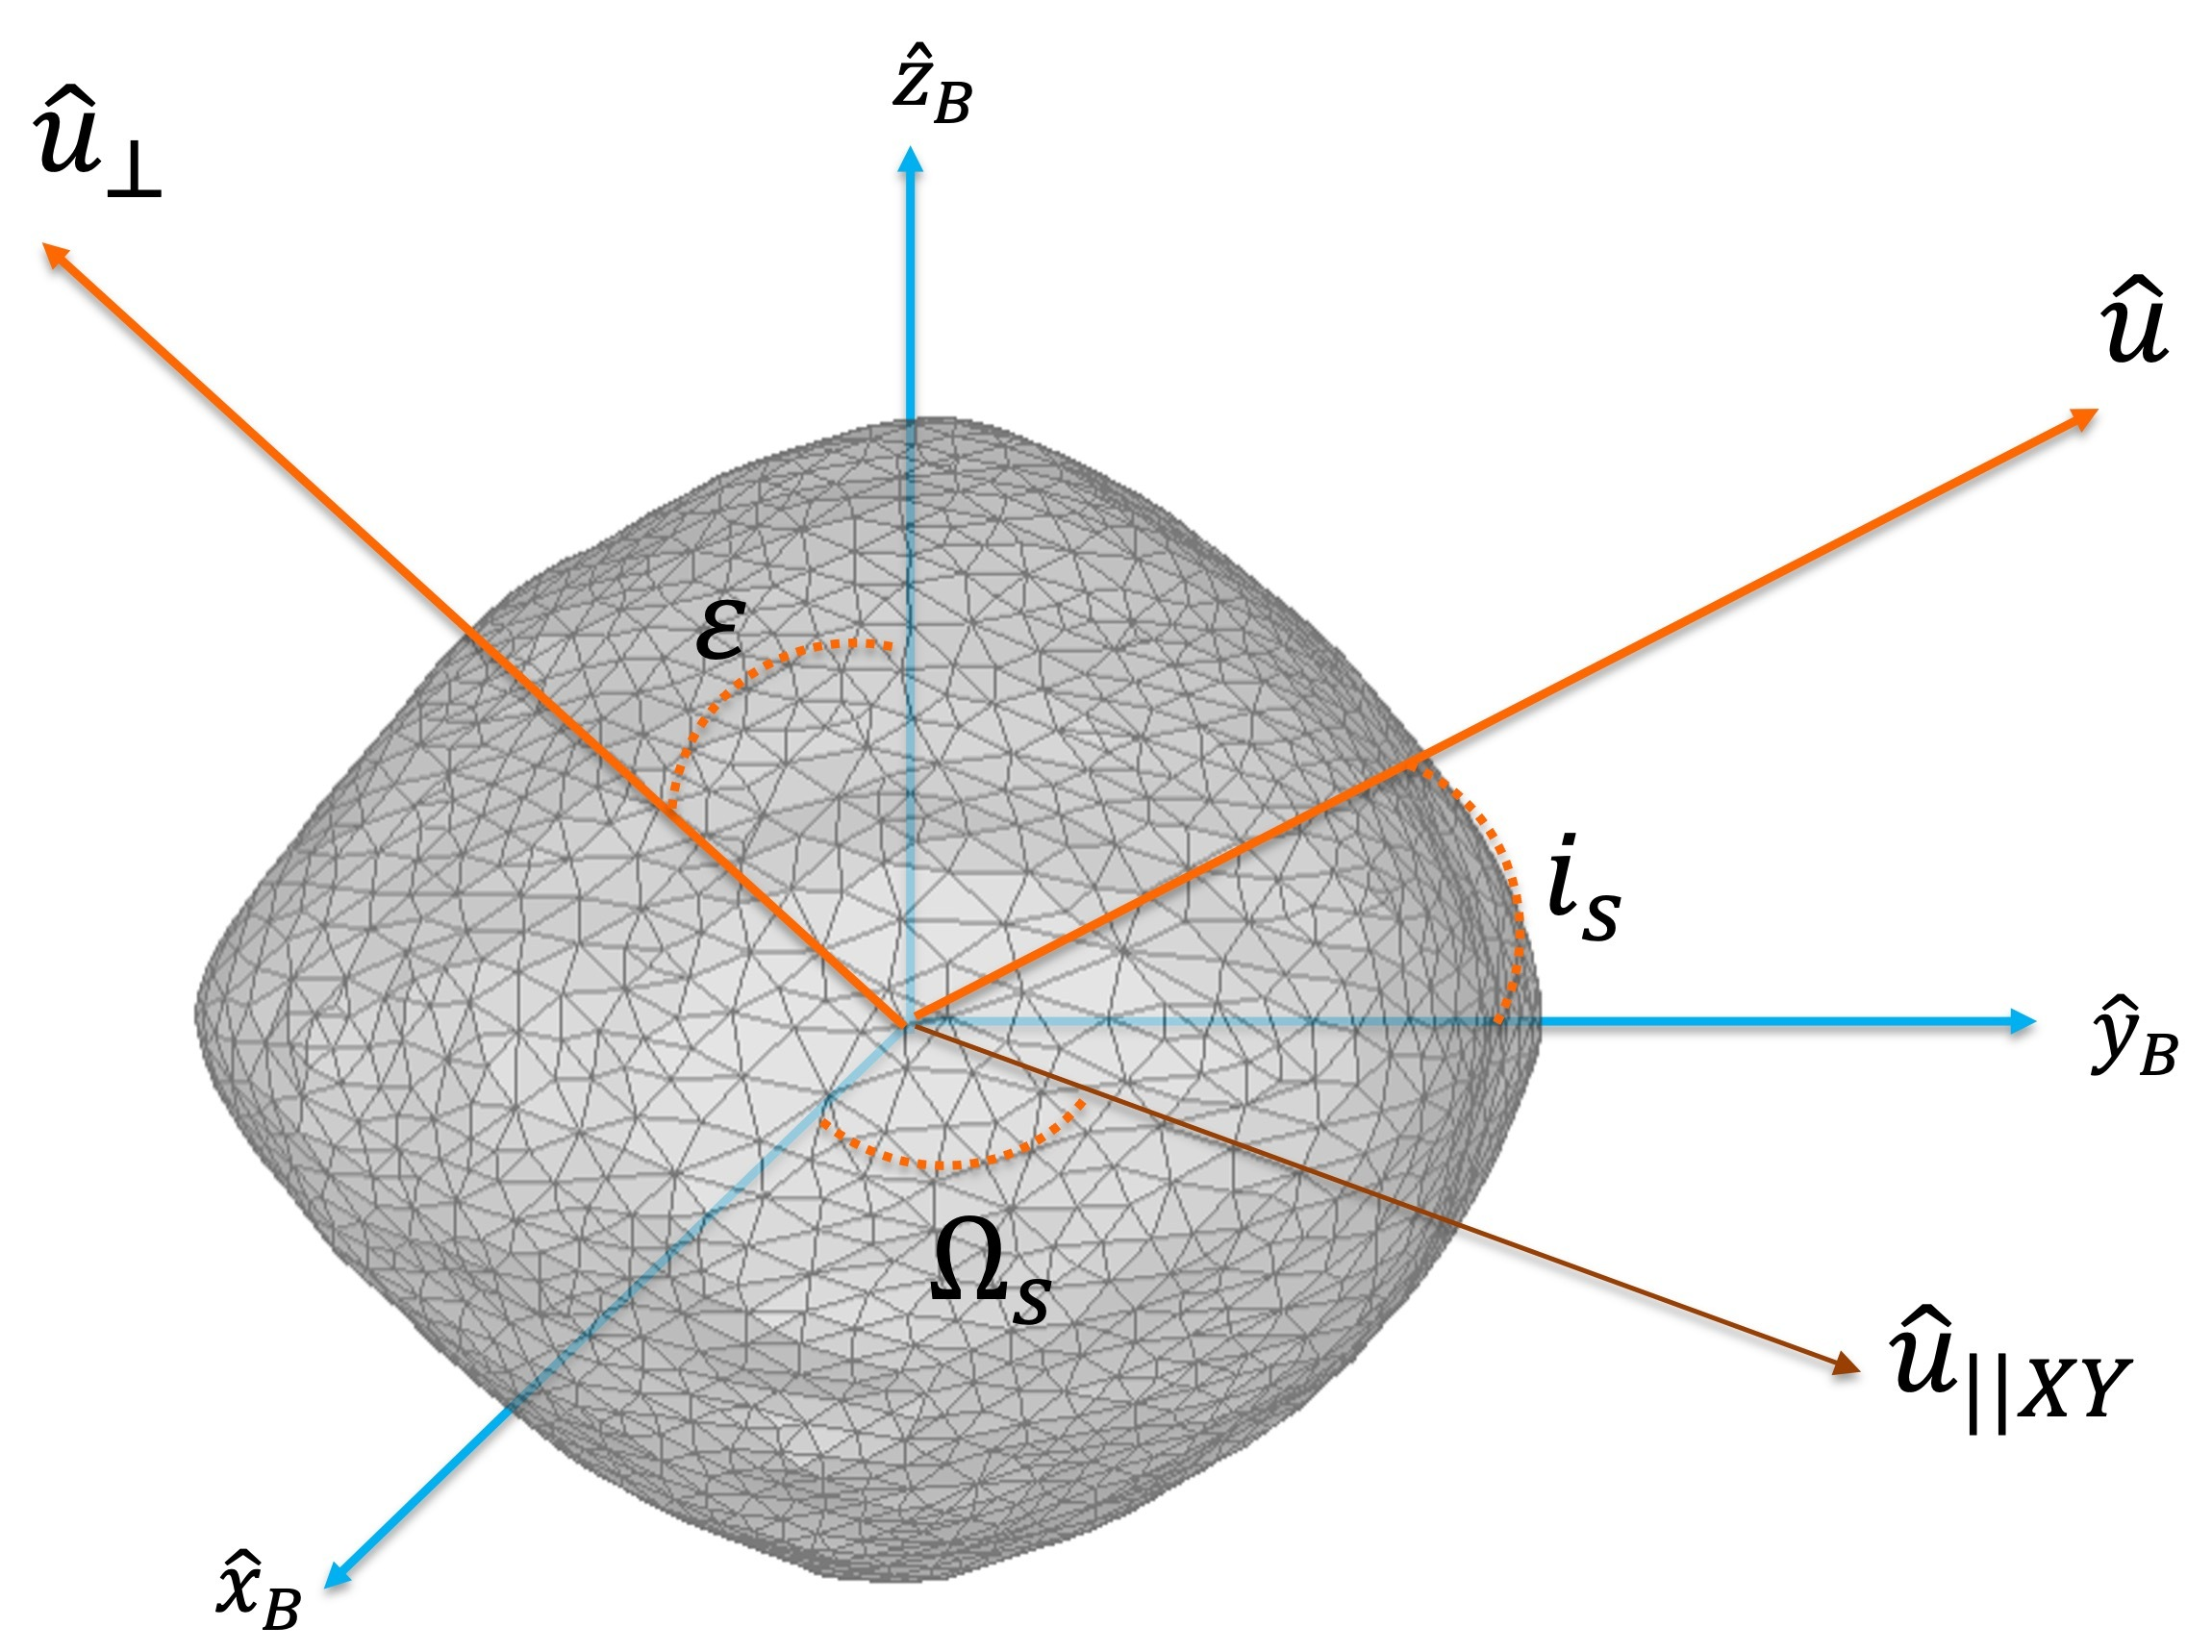
\includegraphics[width=0.5\textwidth]{fig/body_frame_w_obliq.jpg}
%     \caption{Body frame diagram which shows $\hat{u}$, the sun-pointing vector, $\hat{u}_{||xy}$, the projection of the sun-pointing vector into the body x-y plane, $\hat{u}_{\perp}$, the perpendicular vector to the sun-pointing vector, the body frame unit vectors $\hat{x}_B, \hat{y}_B$, and $\hat{z}_B$, as well as the solar inclination angle $i_s$, the longitude of the ascending node $\Omega_s$, and the spin pole obliquity angle $\eta$. }
%     \label{body_frame}
% \end{figure}

\section{YORP Torques for Obliquity} \label{yorp}

%begin here with the basic equations for YORP dynamics like from Golubov Limiting Behavior of Asteroid Obliquity and Spin Using a Semi-analytic Thermal Model of the YORP Effect
%just show how we are approaching the description of YORP torques, including reference to the normalized versions
%\subsection{Fourier YORP Coefficients}
%Here we will reproduce the basic derivation steps from Scheeres, 2007 to present the formulation of YORP torque coefficients that are calculated to find the rate of change of angular velocity and inclination (or obliquity) angle of the asteroid experiencing YORP torque.
%We apply the derivations of Scheeres which used a faceted, spin and orbit averaged approach to calculate fourier coefficients which describe the magnitude of YORP torque. This is derived from assumptions made about the surface, such as low albedo, Lambertian scattering, and uniform rotation. This last assumption can be made for the short periods under which the force equations are averaged, but for the long term periods that we are simulating YORP, this does not apply as we calculate the acceleration of the spin vector over time. The strength of this approach is that we can focus on small contours on the surface and how that changes the overall torque calculations. The forces can be calculated for as small of facets as we can resolve for the surface. That is why we can simulate many small boulders, down to 1 cm in diameter. 

%The coefficients are evaluated from the shape and orbit as follows. We begin by defining the force due to YORP. The force is calculated following the surface geometry, material thermal properties, and illumination patterns and can be expressed as a function of $\lambda$, the general longitude, in a Fourier decomposition about the periodic rotation angle $\phi$. 
%\begin{equation}
%    \begin{split}
%   \frac{\mathbf{F}(\lambda)}{P(R)} &= \sum^{N}_{i=1}\mathbf{f}(\lambda) \\
%    & = \mathbf{A}_0 + \sum^{\infty}_{n=1}[\mathbf{A}_n cos(n\lambda) + \mathbf{B}_n sin(n\lambda)]
%    \end{split}
%\end{equation}
%We leave the initial derivation steps to be explained in the source paper. Here we will print the relevant equations needed for the understanding of our analysis. Next is the expression for the zeroth-order A coefficient which depends on $\rho$, the surface albedo, $s$, the specular reflection ratio, as well as the facet $i$ normal vector $\mathbf{\hat{n}}_i$, the identity dyad $\mathbf{U}$, the thermal coefficient $a_2 = B(1-s)\rho + (1-\rho)B$ where $B$ is the Lambertian scattering coefficient assumed to be 2/3, and the illumination integrals $\mathbf{I}$ with bounds equal to the rise and set longitudes (defined in Scheeres'). We present the equation for $A_0$ and leave it to the reader to find the equivalent expressions for higher order terms and the B coefficient.   
%\begin{equation}
%     \begin{split}
%     \mathbf{A}_{0,i} = &\frac{A_i}{2\pi} \Big[\Big\{\rho s (2\mathbf{\hat{n}}_i\mathbf{\hat{n}}_i - \mathbf{U}) +\mathbf{U}  \Big\}\cdot \mathbf{I}^2_{c0,i} \cdot \mathbf{\hat{n}}_i \\
%     & + a_2 \mathbf{\hat{n}}_i \mathbf{\hat{n}}_i \cdot \mathbf{I}^1_{c0,i}\Big]
%     \end{split}
% \end{equation}
% While $A_0, A_1$, and $B_1$ are the decomposed coefficients of the force expression, the moment coefficients follow the same relationship as force and moment themselves. Therefore we find $C_{n,i}$ and $D_{n,i}$ with the simple cross product. 
% \begin{equation}
%     \mathbf{C}_{n,i} = \mathbf{r}_i \times \mathbf{A}_{n,i}
% \end{equation} 
% \begin{equation}
%     \mathbf{D}_{n,i} = \mathbf{r}_i \times \mathbf{B}_{n,i}
% \end{equation}
The equations of motion overall are the spin rate, spin acceleration, change in solar inclination, and change in solar longitude of the ascending node. These last two are substitutes for obliquity angle and right ascension of the pole direction. While solar inclination and longitude are parameterized in the body fixed frame, the obliquity and right ascension are properties of the orbit in the inertial frame. We continue with body-fixed parameters in order express our motion due to the local body-incident forces of YORP. As we've already reviewed spin rate dynamics in the previous chapter, we will reproduce the pole tilt equations of motion here for reference.

% \begin{equation}
%     \dot{\phi} = \omega
% \end{equation}
% \begin{equation}
%     \dot{\omega} = \mathit{W}_B \:\bar{C}_{0,z}(i)
% \end{equation}
\begin{equation}
    \begin{split}
    \dot{i} = \:&\frac{\mathit{W}_B}{\omega}\Big[(\bar{C}_{1,x}(i)+\bar{D}_{1,y}(i))\: \cos(\omega T_{lag}) \\
    & + (\bar{D}_{1,x}(i)-\bar{C}_{1,y})\: \sin(\omega T_{lag})\Big]
    \end{split}
\end{equation}
\begin{equation}
    \begin{split}
    \dot{\Omega} = &-\frac{cot(i)\mathit{W}_B}{\omega}\Big[- (\bar{D}_{1,x}(i)-\bar{C}_{1,y}(i)) \:\cos(\omega T_{lag}) \\
    & + (\bar{C}_{1,x}(i)+\bar{D}_{1,y}) \:\sin(\omega T_{lag})\Big]
    \end{split}
\end{equation}
The term $W_B$ stands for the fraction $G_1 \symbol{92} I_z a^2 \sqrt(1-e^2)$, and is substituted here to further highlight the emphasis on the YORP Fourier coefficients. 

Thermal inertia is approximated in these equations of as a constant time lag, serving to delay the time of emitted energy by some fraction of the period, and in this work we will apply a time lag of 1/8th of the asteroid's currently measured rotation period. This constant time lag ignores the variations in materials of the surface or inertia as a function of spin velocity or time of local day. However, it is useful in these twice averaged equations of motion and allows thermal lag to be isolated in trigonometric terms that scale the first-order YORP torque coefficients. In the next section we will discuss alternative approaches to thermal inertia considerations within these equations. 

%\subsection{YORP Timescales and Spin Limits}
%The YORP timescale ($\tau_Y$) refers to the amount of time it takes for the angular velocity to double or halve as a result of YORP-induced acceleration, and it analytically defined as the current spin rate divided by the spin acceleration. 
%\begin{equation}
%    \frac{\omega}{\dot{\omega}} = \tau_Y = \frac{4\pi A^2\sqrt{1-E^2}}{3\Phi} \frac{\omega \rho R^2}{\mathit{C}}
%\end{equation}
%This is defined by Scheeres and Sanchez, and applies Scheeres notation for YORP spin acceleration \citep{Scheeres2014}\citep{Scheeres2007}. Mentioning these barriers to YORP dynamics is important because the original intention of defining the YORP effect was to explain how small meteroids are accelerated to the point of disruption \citep{Rubincam2000}. We extend it to small rubble-pile asteroids to explain the unmodeled accelerations observed in their dynamics.
%This delimiter of time is important for tracking how quickly YORP is changing the dynamics and it can tell us how often to expect the body to go through a complete "YORP cycle", or period of accelerating up to a breakdown speed and then rearranging until slower, stable angular velocity is achieved \citep{Scheeres2019}. This is the typical cycle for a body with positive YORP torques, but we can see a similar cycle with YORP spin-down and tumbling. These are idealized versions of the stochastic events that we predict for YORP evolution so we assume secular acceleration and non-dynamic surfaces when defining this behavior. We will show here the angular velocity requirements for disaggregation as well as for tumbling. Tumbling requires that there are non-periodic forces impacting the obliquity evolution term. %check this

%There are two velocities relevant for rotational fission. The first is the spin rate at which deformation begins, when the cohesive forces are overcome by the centrifugal forces at the surface. The second is the failure spin rate, where plastic deformation is induced. This goes beyond the cohesiveless spin rate $\omega_c$ \citep{Scheeres2018}\citep{Sanchez2014}.
% \begin{equation}
%     \omega_{c} = \sqrt{\frac{4\pi \mathit{G}\rho}{3}}
% \end{equation}
% \begin{equation}
%     \omega^2_F = \omega^2_c + \frac{2\sigma}{\rho \alpha^2} \frac{3 - sin \phi}{3 + sin \phi}
% \end{equation}
%tumbling

%Below in table \ref{table:properties} are the physical constants used to determine the cohesive force barrier velocity and failure spin rates. %I need G, I don't think it's the constant that I think it is. the units don't work

% \begin{table}[H]
%     \renewcommand{\arraystretch}{1.5}

%     \resizebox{\textwidth}{!}{
%         \begin{tabular}{| c || c | c | c | c | c |}
%         \hline
%         \makegapedcells
%         \textbf{Body} & \textbf{Density}, $\rho$ & \textbf{Cohesive Strength}, $\sigma$ & \textbf{Longest Radius}, $\alpha$ & \textbf{Angle of Friction},$\phi$ \\
%         \hline 
%         \hline
%         \makegapedcells
%         Bennu & 1260 $kg/m^3 $ \citep{Chesley2014} & 1 Pa \citep{Walsh2022} & 282.37 m & $35^{\circ}$ \citep{Zhang2022} \\ 
%         \hline 
%         \makegapedcells 
%         Itokawa & 2000 $kg/m^3$ \citep{Sanchez2014} & 25 Pa \citep{Sanchez2014}  & 267.5 m & 40 \citep{Aoki2014}\\  
%         \hline   
%         \end{tabular}
%         }
%     \caption{Granular properties for asteroid disaggregation limits}
%     \label{table:properties}
% \end{table}

%another plot of likeeeeeeeeee YORP timescales?
%\subsection{Thermal Modeling}
%%%%%%%%%%%
%%%%%%%%%%%
%%%%%%%%%%%%%% ANALYSIS NEEDED %%%%%%%%%%%%%%%%%%%%%%%%%%%%%%%%%%%%%%%%%%%%%%%%%%
%%%%%%%%%%%
%%%%%%%%%%%

%now present the logic of the constant thermal lag, compare it to the thermal parameter. At the end sprinkle in the thermal lag on order of period analysis
%\subsubsection{Constant Thermal Lag Assumption}

%\subsection{Stochastic Thermal Lag}
%%%%%%%%%%%
%%%%%%%%%%%
%%%%%%%%%%%%%% ANALYSIS NEEDED %%%%%%%%%%%%%%%%%%%%%%%%%%%%%%%%%%%%%%%%%%%%%%%%%%
%%%%%%%%%%%
%%%%%%%%%%%

%do a quick analysis showing what happens if you just make each facet a random time lag varied from an initial value of T/8
%can I simulate what happens if I uncover a lighter patch of material with different thermal inertia than the original regolith? simulating what happened when osiris-rex sampled the surface of Bennu

%\subsubsection{Time-Varying Thermal Inertia}
%list out the assumptions we will still make in this model
%how does this compare to the way other people are doing it?
%time of day variation and accumulation. Wouldn't it be sensitive to choice in initial orientation of the prime meridian?
%%%%%%%%%%%
%%%%%%%%%%%
%%%%%%%%%%%%%% ANALYSIS NEEDED %%%%%%%%%%%%%%%%%%%%%%%%%%%%%%%%%%%%%%%%%%%%%%%%%%
%%%%%%%%%%%
%%%%%%%%%%%

%\section{Spin and Stability Dynamics} \label{spin}

%The asteroid dynamics that YORP is acting upon can be summarized with the phase angle, $\phi$, the rotational velocity, $\omega$, the solar inclination, $i_s$, and the solar longitude, $\Omega_s$. These are all variables in the body fixed frame. We will also consider the euler parameters of the attitude of the spin pole in order to track orientation over time in the inertial frame. The full dynamical state space is given below.%below give all the equations and dynamics

%\begin{equation}
%    [] = []
%\end{equation}

%We propagate these dynamics using the rotational motion equations as well as the ones defined as influenced by YORP. This could be expanded to include natural phenomena such as SRP, but we will remain focused here on just the YORP torque contributions to the dynamics over time. The goal is to evaluate how much the YORP timescale is changed, and how the stability of the pole is altered. In simulating both in tandem, we can find whether the body will secularly accelerate in spin to an end-state or if the requirements for tumbling motion are met before this can occur. 
%%%%%%%%%%%
%%%%%%%%%%%
%%%%%%%%%%%%%% ANALYSIS NEEDED %%%%%%%%%%%%%%%%%%%%%%%%%%%%%%%%%%%%%%%%%%%%%%%%%%
%%%%%%%%%%%
%%%%%%%%%%%

%Now we talk about the figure above. 
      

%We will begin our stability analysis by describing this homogenous system. This assumption makes it applicable to use the same YORP coefficients throughout. The general solution for the state in this form is as follows. 

%\begin{equation}
%    \centering
%    \mathbf{x}(t) = e^{[A](t-t_0)}\mathbf{x}(t_0)
%\end{equation}
%We will follow the format of \citep{Schaub2018} to describe the sensitivity matrix. This is to analyze the sensitivities of the current state vector to variations in the initial state vector. This follows our analysis of the sensitivity of spin dynamics to the changes induced by boulders. 

%There are three types of stability that could be applied to this problem. Euclidean, Lagrange, and Lyapunov. Because we care about the initial conditions and staying near them in the long term, we will use Lyapnov stability methods to analyze the behavior of an asteroid spinning under the influence of YORP accelerations in the obliquity angle.

%We now apply Lyapunov's direct method to study the stability of this system in it's current formulation. 


%We will also look at the asymptotic stability because we care about these bodies asymptotically approaching an end-state. 
%show phase space diagram of x(t) as x axis and \dot(x)(t) as the y axis

\section{Results} \label{results}
%show the way the results change with varying thermal models
%it would be cool to have color plots of surface with different thermal parameters
%could I randomize thermal parameter by facet?
%no separate sections for bennu and itokawa
\subsection{Boulder Distribution Effects on Solar Inclination Change Rates}
We find that for each combination of 5000 randomly selected boulders, scaled proportionally by the size distribution which is also randomly but sufficiently sampled from, we find significant variability in the solar inclination torque. We will also map this to the additional west/east surface area that is applied through this procedure. Sensitivity of the YORP effect to the individual boulders is tested by isolating the boulders that contribute more than 1\% to the total inclination torque magnitude. This is then analyzed for the distribution in size, orientation, and location.

We have calculated the sum of the torque influence from each boulder and present it in Fig. \ref{fig:is_results} for both the asteroid Bennu and Itokawa shapes. For N=500 cases, we see different variance in each case. While most of the cases have close to zero change in the obliquity shifting rate due to boulders, we see a handful of cases that deviate towards the maximum influences of 2e-12 and 5e-12, for Bennu and Itokawa respectively. In the following subsections, we will show the significance of certain properties of boulders and what the distributions of the most influential individuals looks like.

\begin{figure}
    \begin{subfigure}{0.49\textwidth}
        \centering
        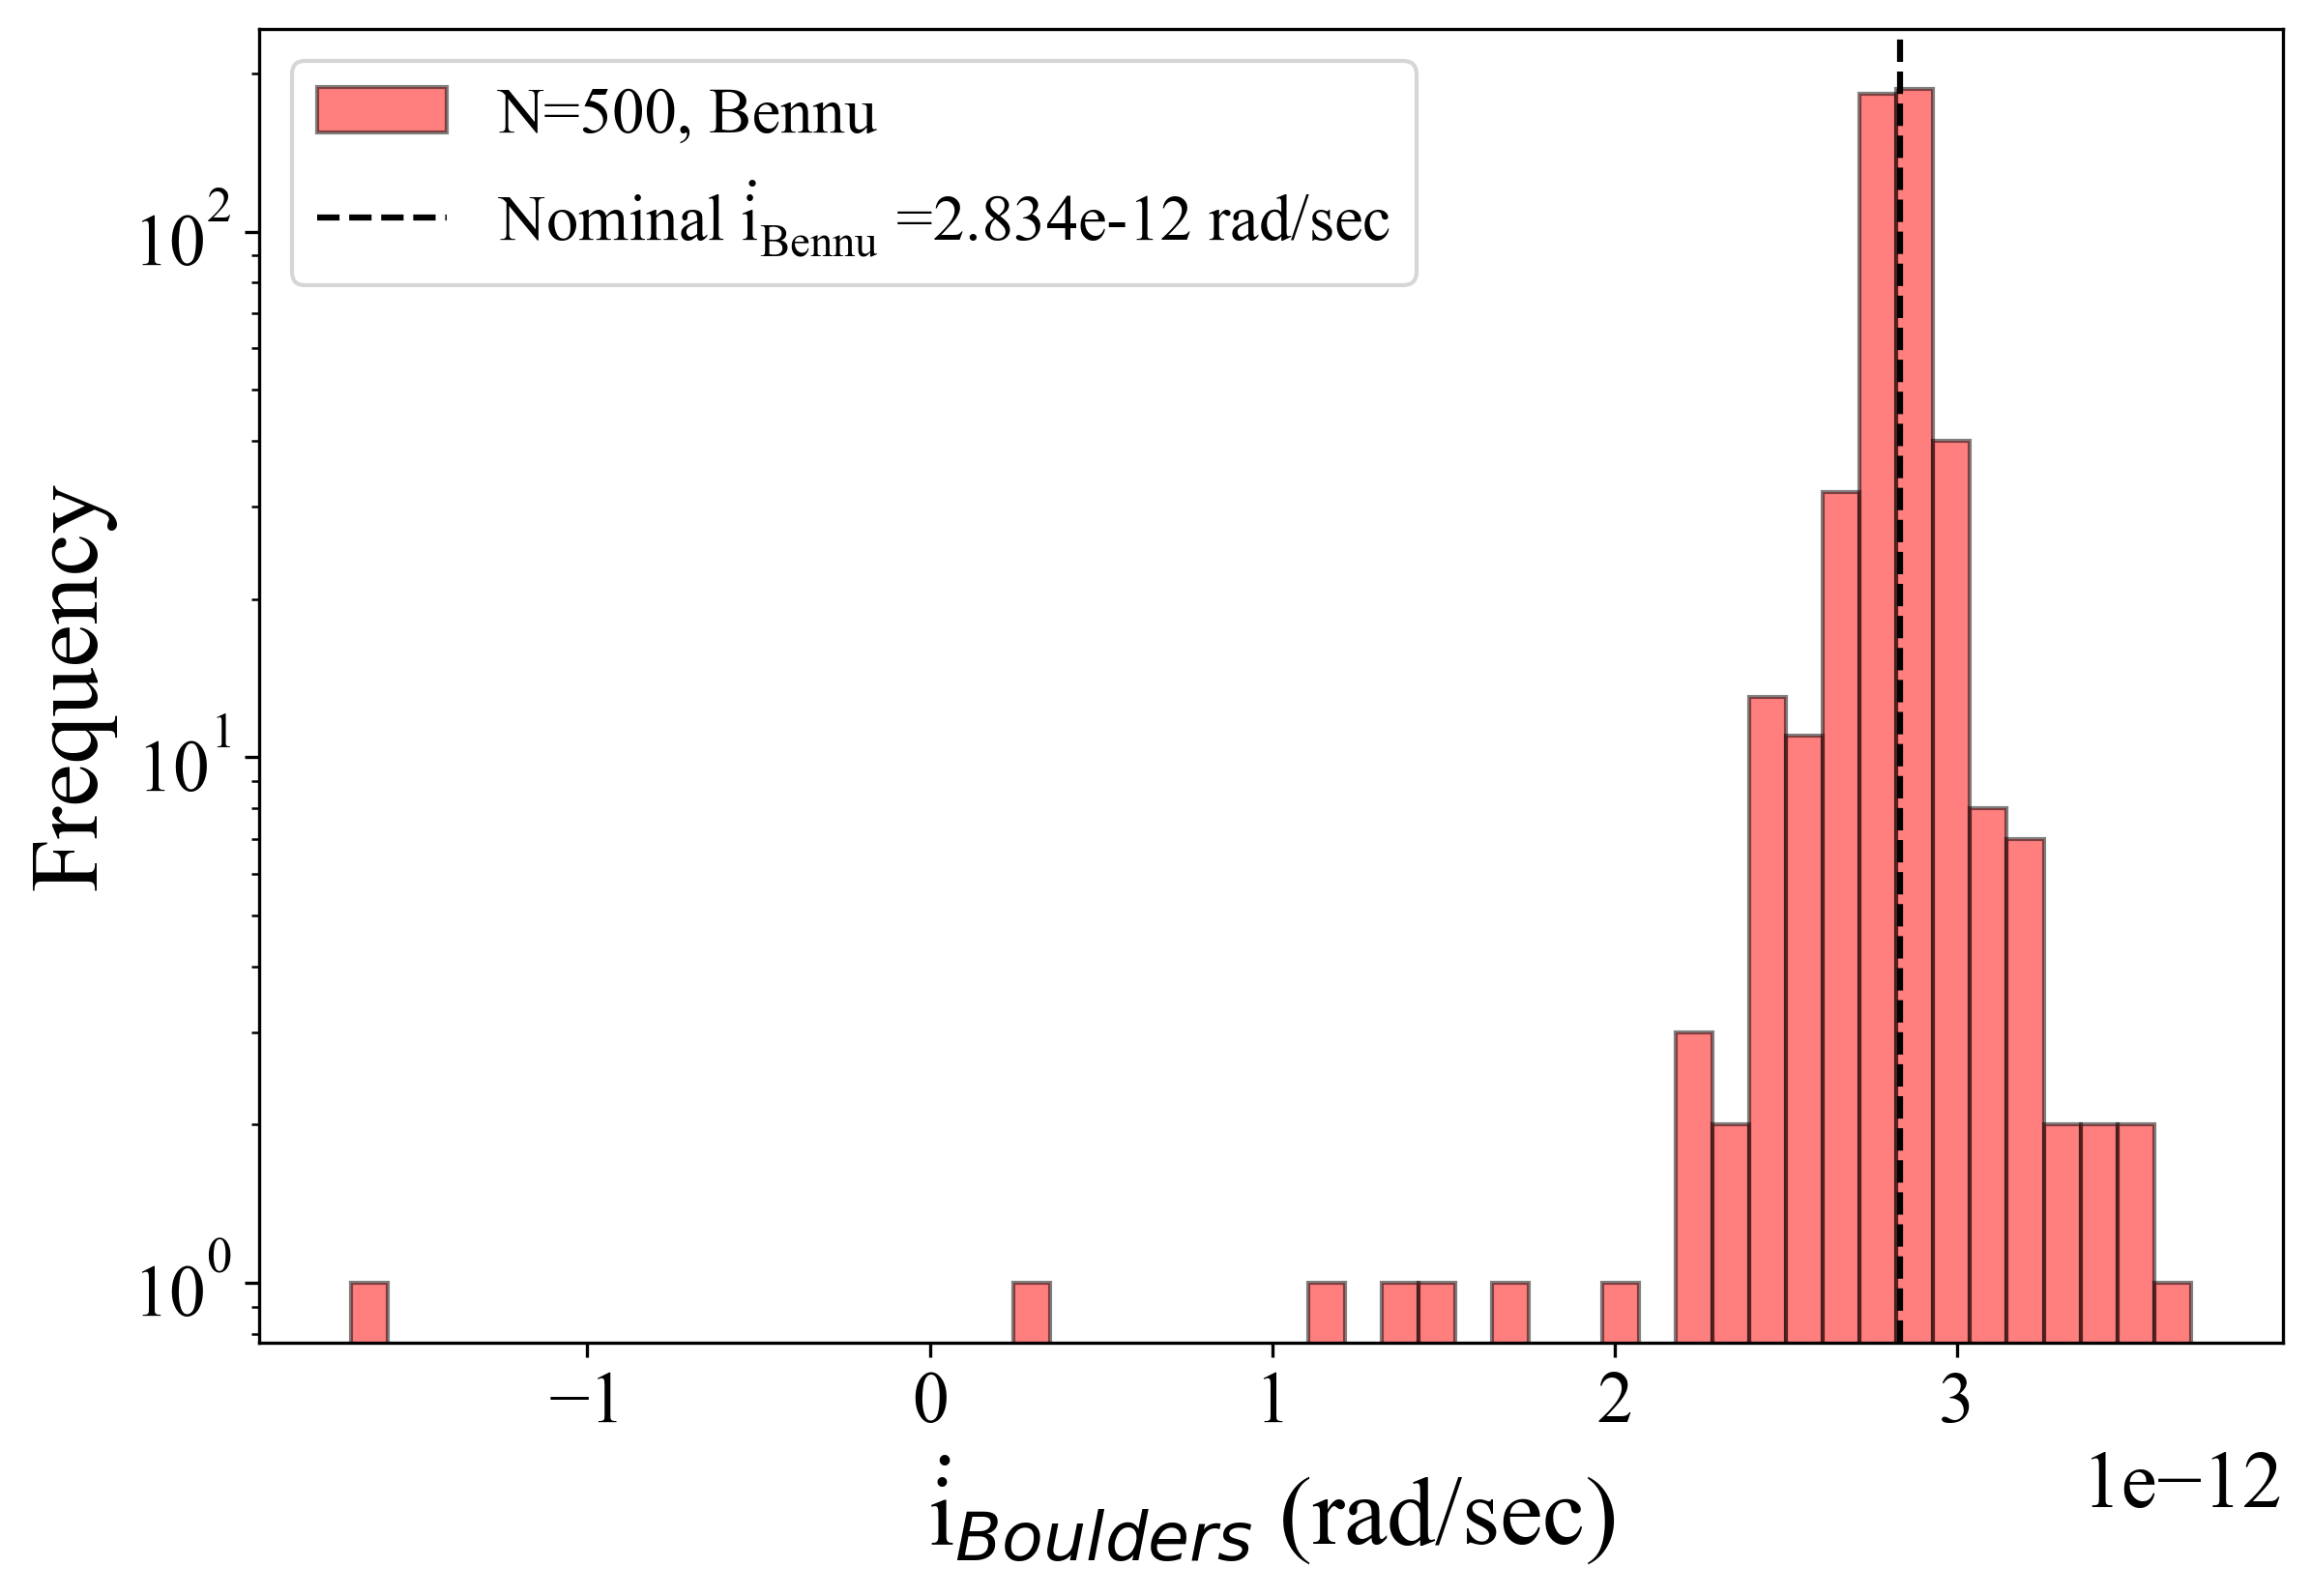
\includegraphics[width=\textwidth]{fig/initial_obliq_dot_dist_bennu.png}
        \caption{Distribution of Global Solar Inclination Rate due to Added Boulders on Bennu, 500 cases}
    \end{subfigure}
    \hfill
    \begin{subfigure}{0.49\textwidth}
        \centering
        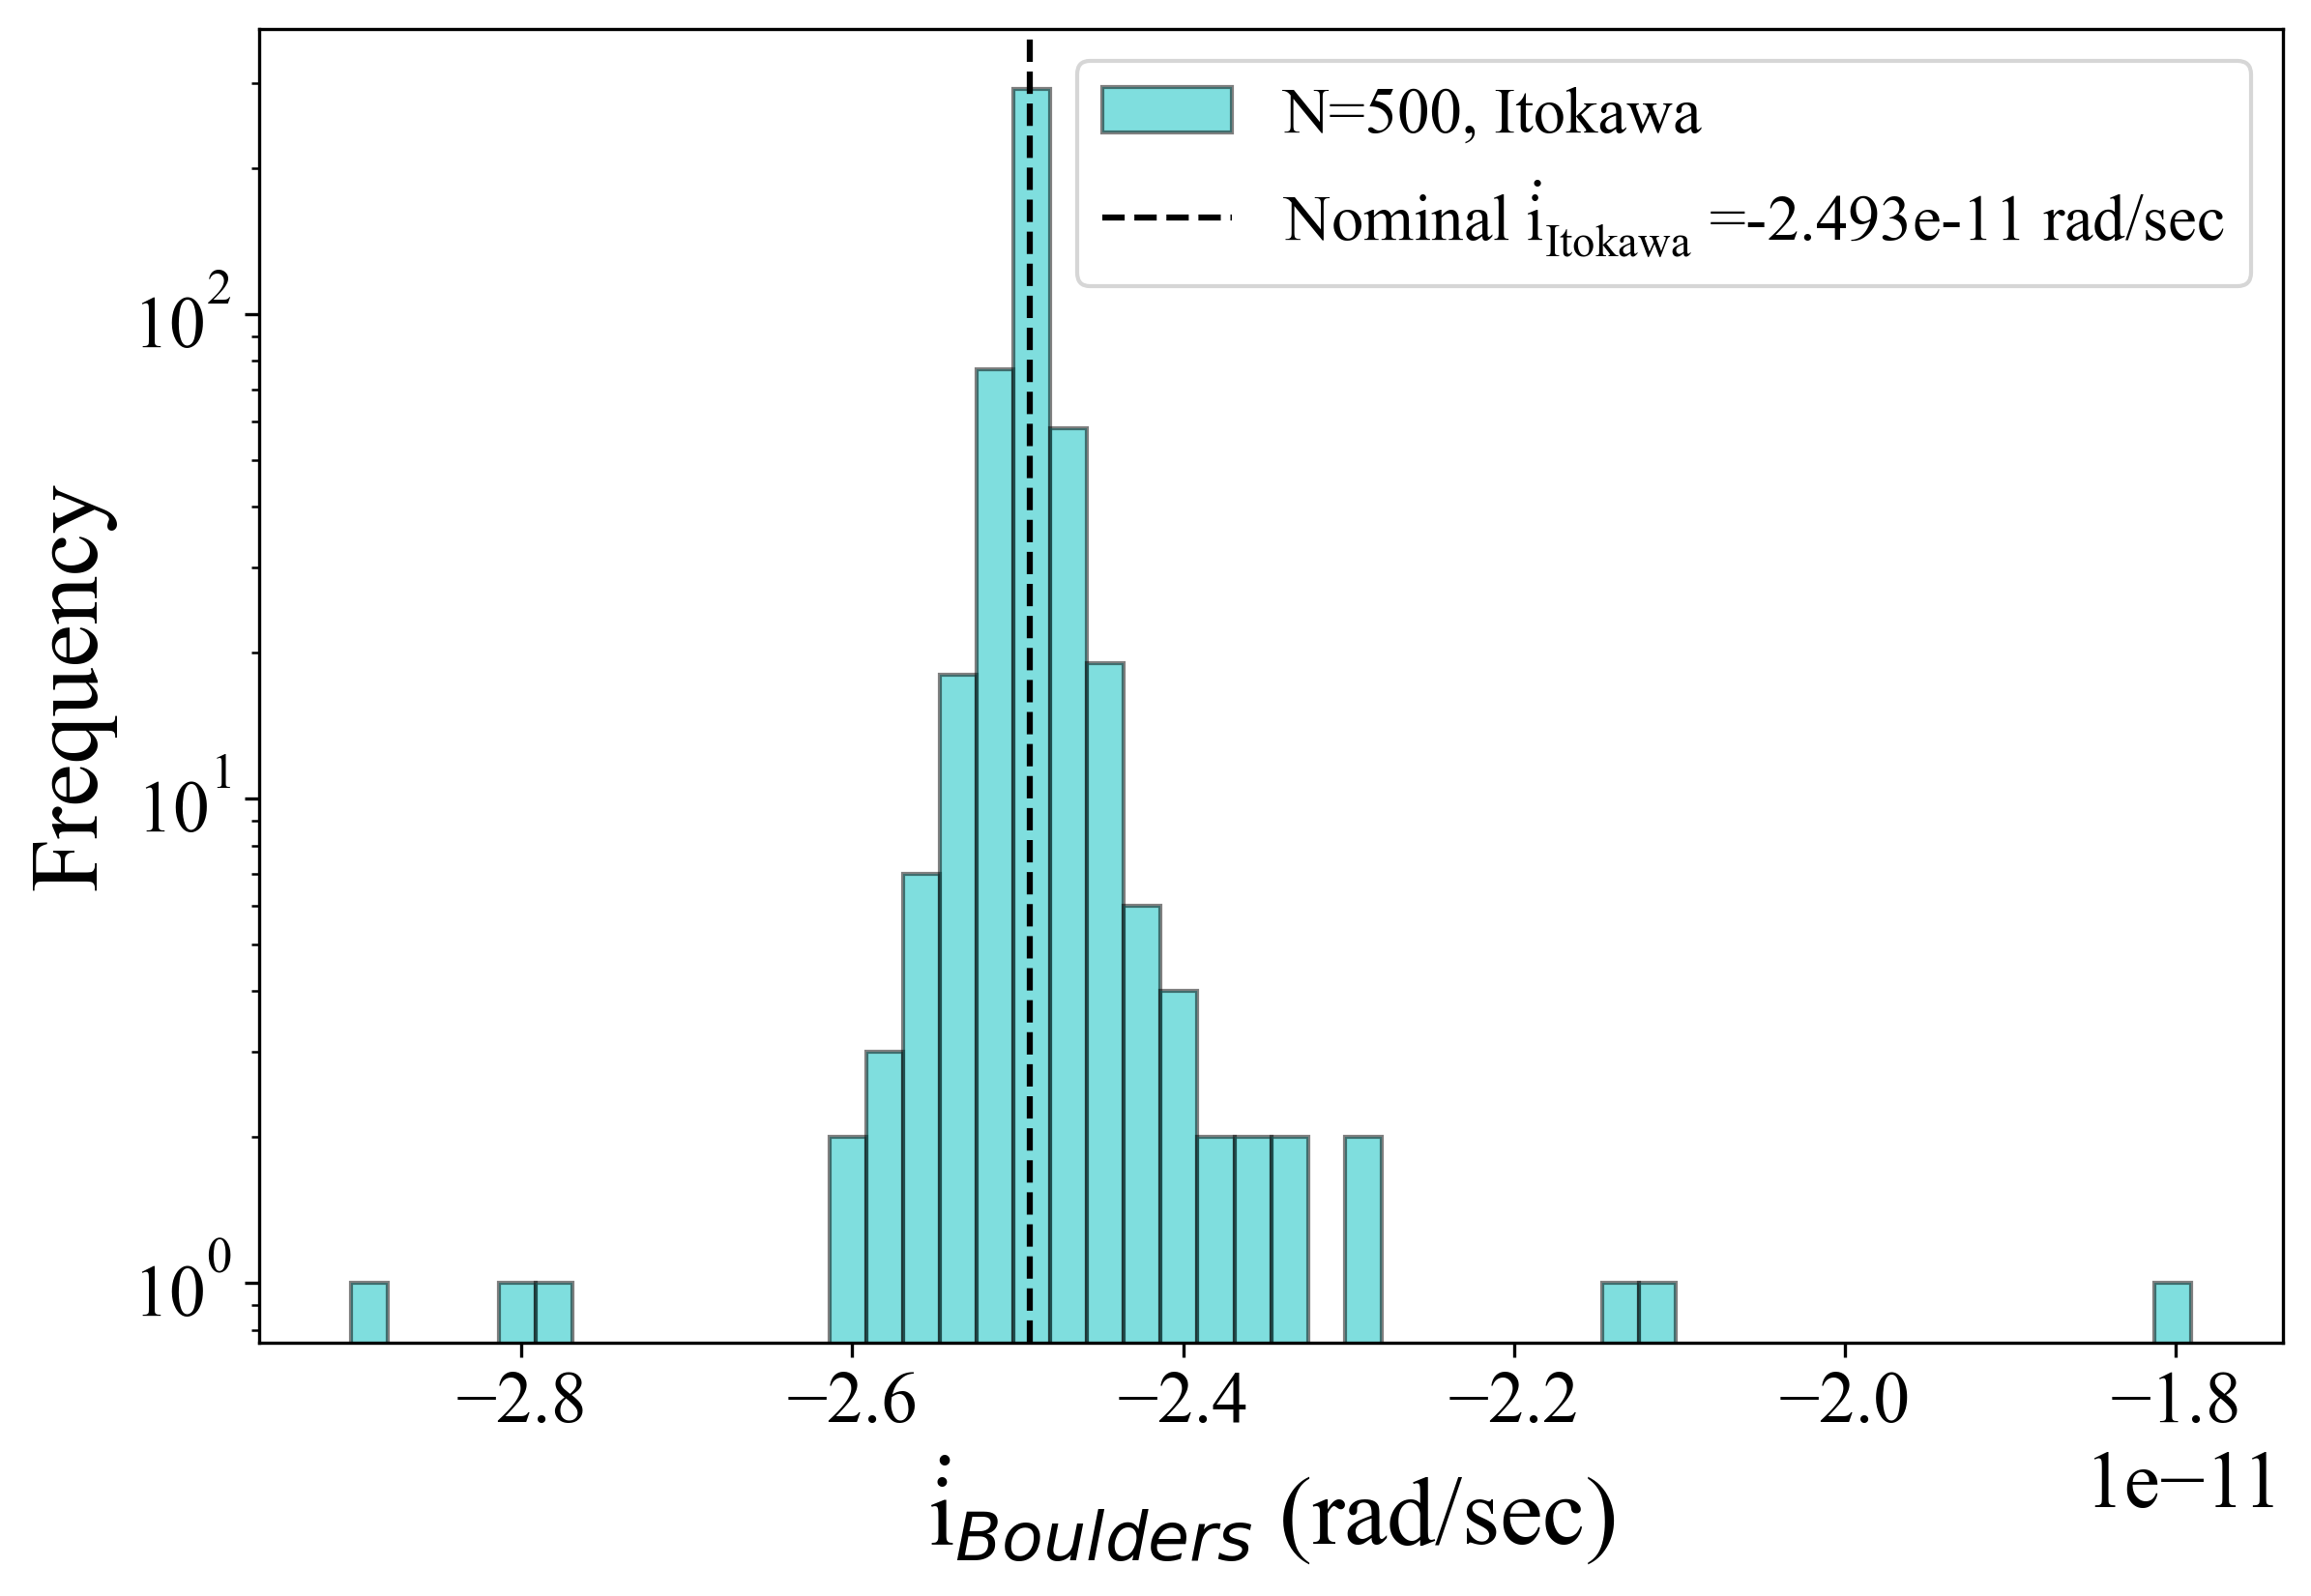
\includegraphics[width=\textwidth]{fig/initial_obliq_dot_dist_itokawa.png}
        \caption{Distribution of Global Solar Inclination Rate due to Added Boulders on Itokawa, 500 cases}
    \end{subfigure}  
    \caption{Solar Inclination Rates for entire asteroid with 5000 boulders added in 500 different configurations of size, orientation, and location on Bennu and Itokawa shape models}
    \label{fig:is_results}
\end{figure}


\subsection{Sensitivity}

We have applied the characterizations of the size power law of boulders on Bennu and Itokawa that come from image-based analysis due to the OSIRIS-REx and Hayabusa missions. The size of each boulder selected randomly for surface placement was sampled from this power law, modeled by the dashed lines in Fig. \ref{fig:all_size}. The histogram shows the full distribution of every size boulder selected for this simulation study. Now we will separate the population by which boulders contribute over $1\%$ to the obliquity changing rate despite each representing a constituency of $0.02\%$ percent of the population. 


Now comparing Fig. \ref{fig:all_size} and Fig. \ref{fig:size_onepercent}, we see that the boulders smaller than 0.01m in diameter begin to be lost when filtering for large contributions to YORP obliquity change. It's the same result independent of the underlying shape.



\begin{figure}[H]
    \begin{subfigure}{0.49\textwidth}
        \centering
        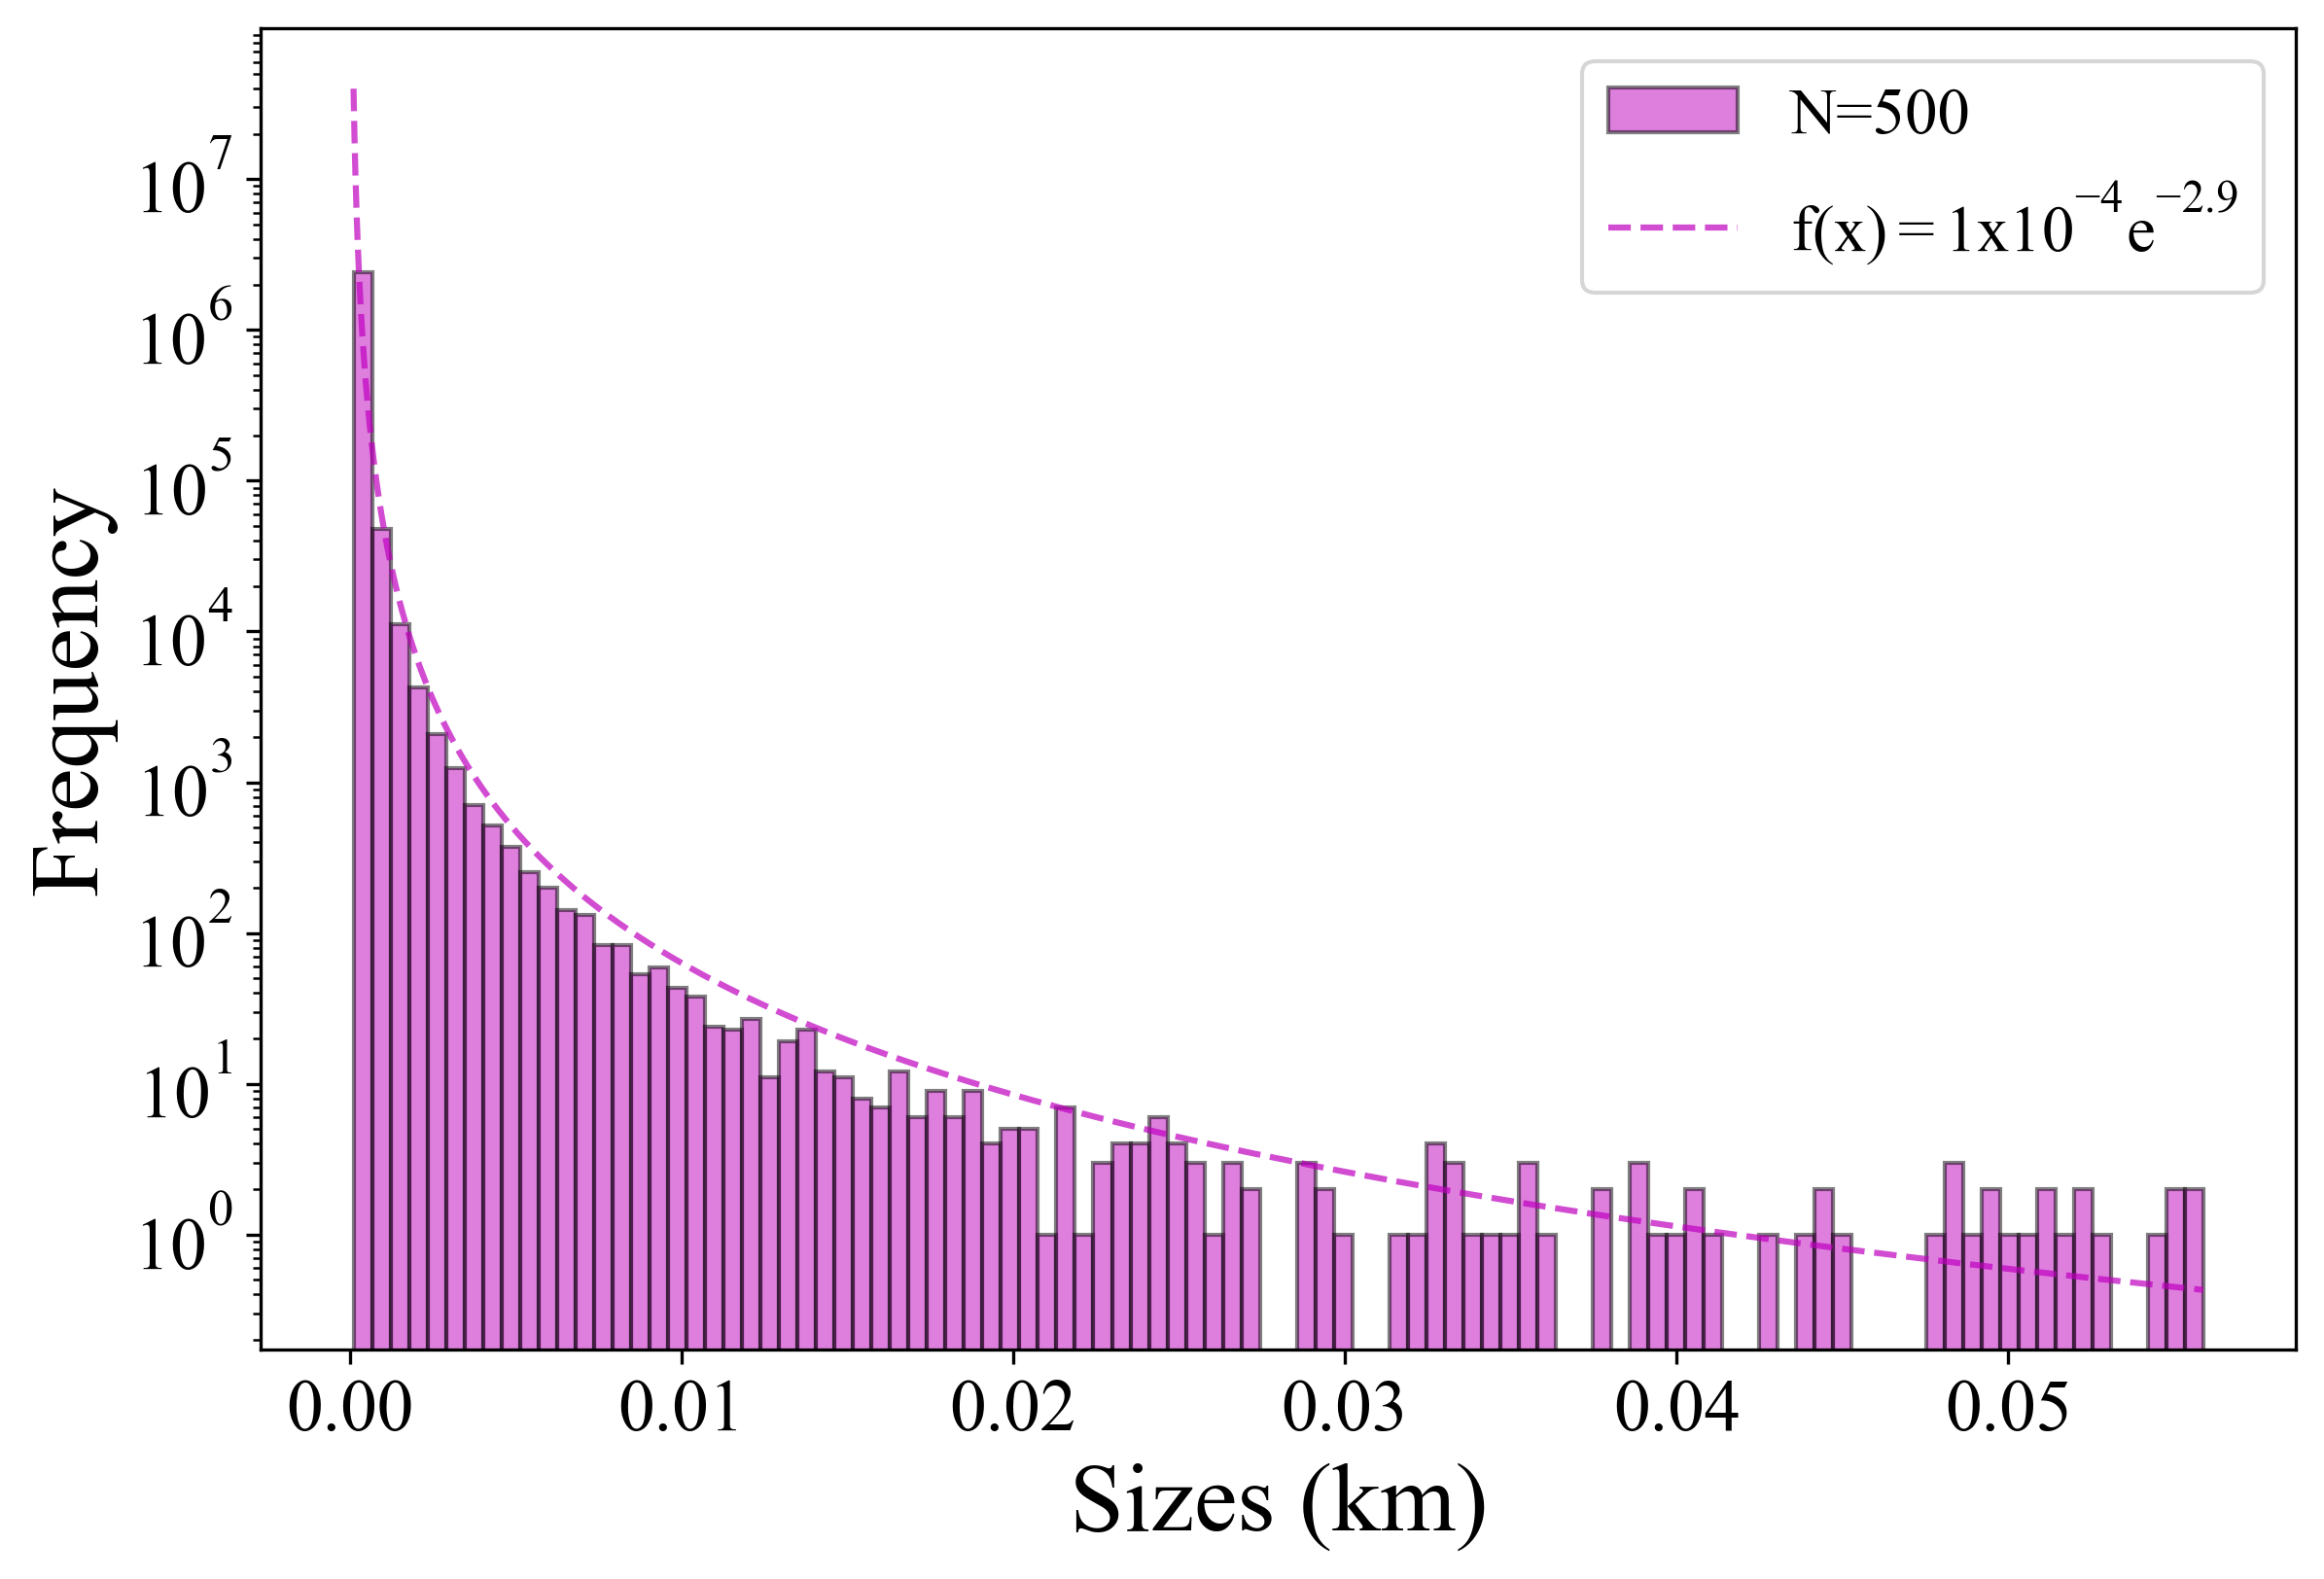
\includegraphics[width=\textwidth]{fig/boulder_size_dist_bennu.png}
        \caption{Power law size distribution for Bennu in theory and sampled, $\alpha$ = -2.9}
    \end{subfigure}
    \hfill
    \begin{subfigure}{0.49\textwidth}
        \centering
        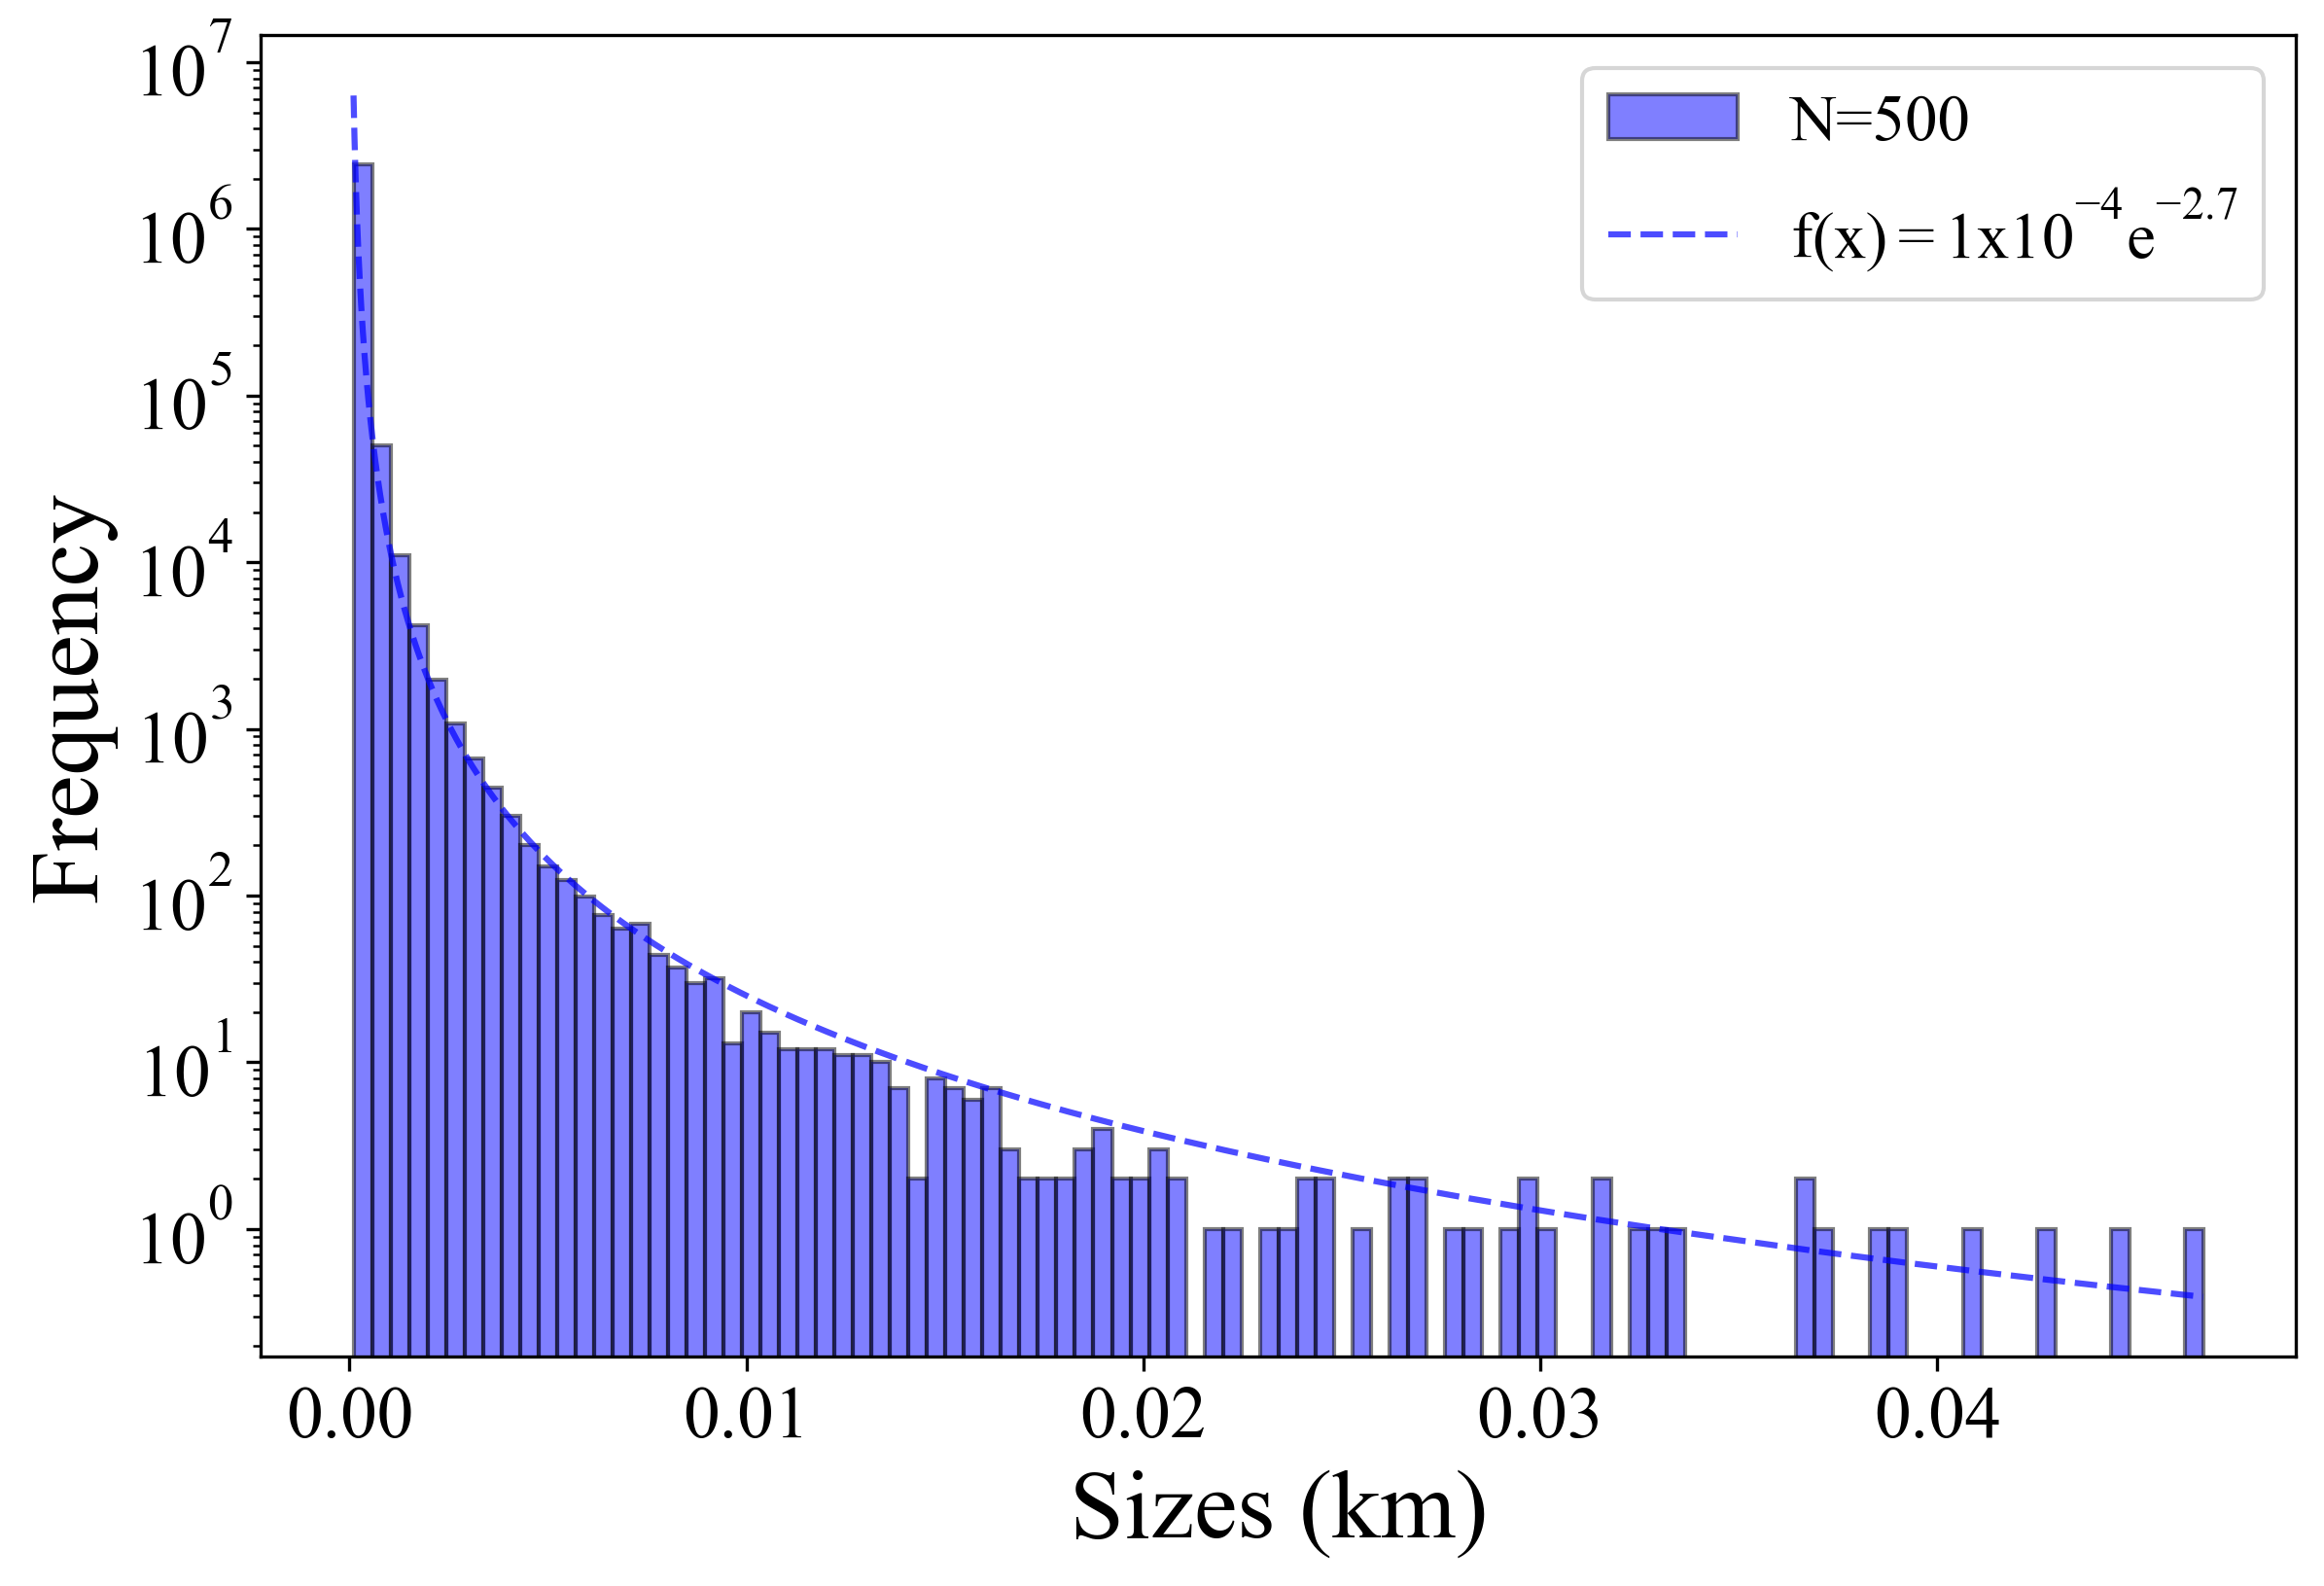
\includegraphics[width=\textwidth]{fig/boulder_size_dist_itokawa.png}
        \caption{Power law size distribution for Itokawa in theory and sampled, $\alpha$ = -2.7}
    \end{subfigure}  
    \caption{Boulder diameter power laws: dashed line is the model and histogram represents the population sampled from power law}
    \label{fig:all_size}
\end{figure}

\begin{figure}[H]
    \begin{subfigure}{0.49\textwidth}
        \centering
        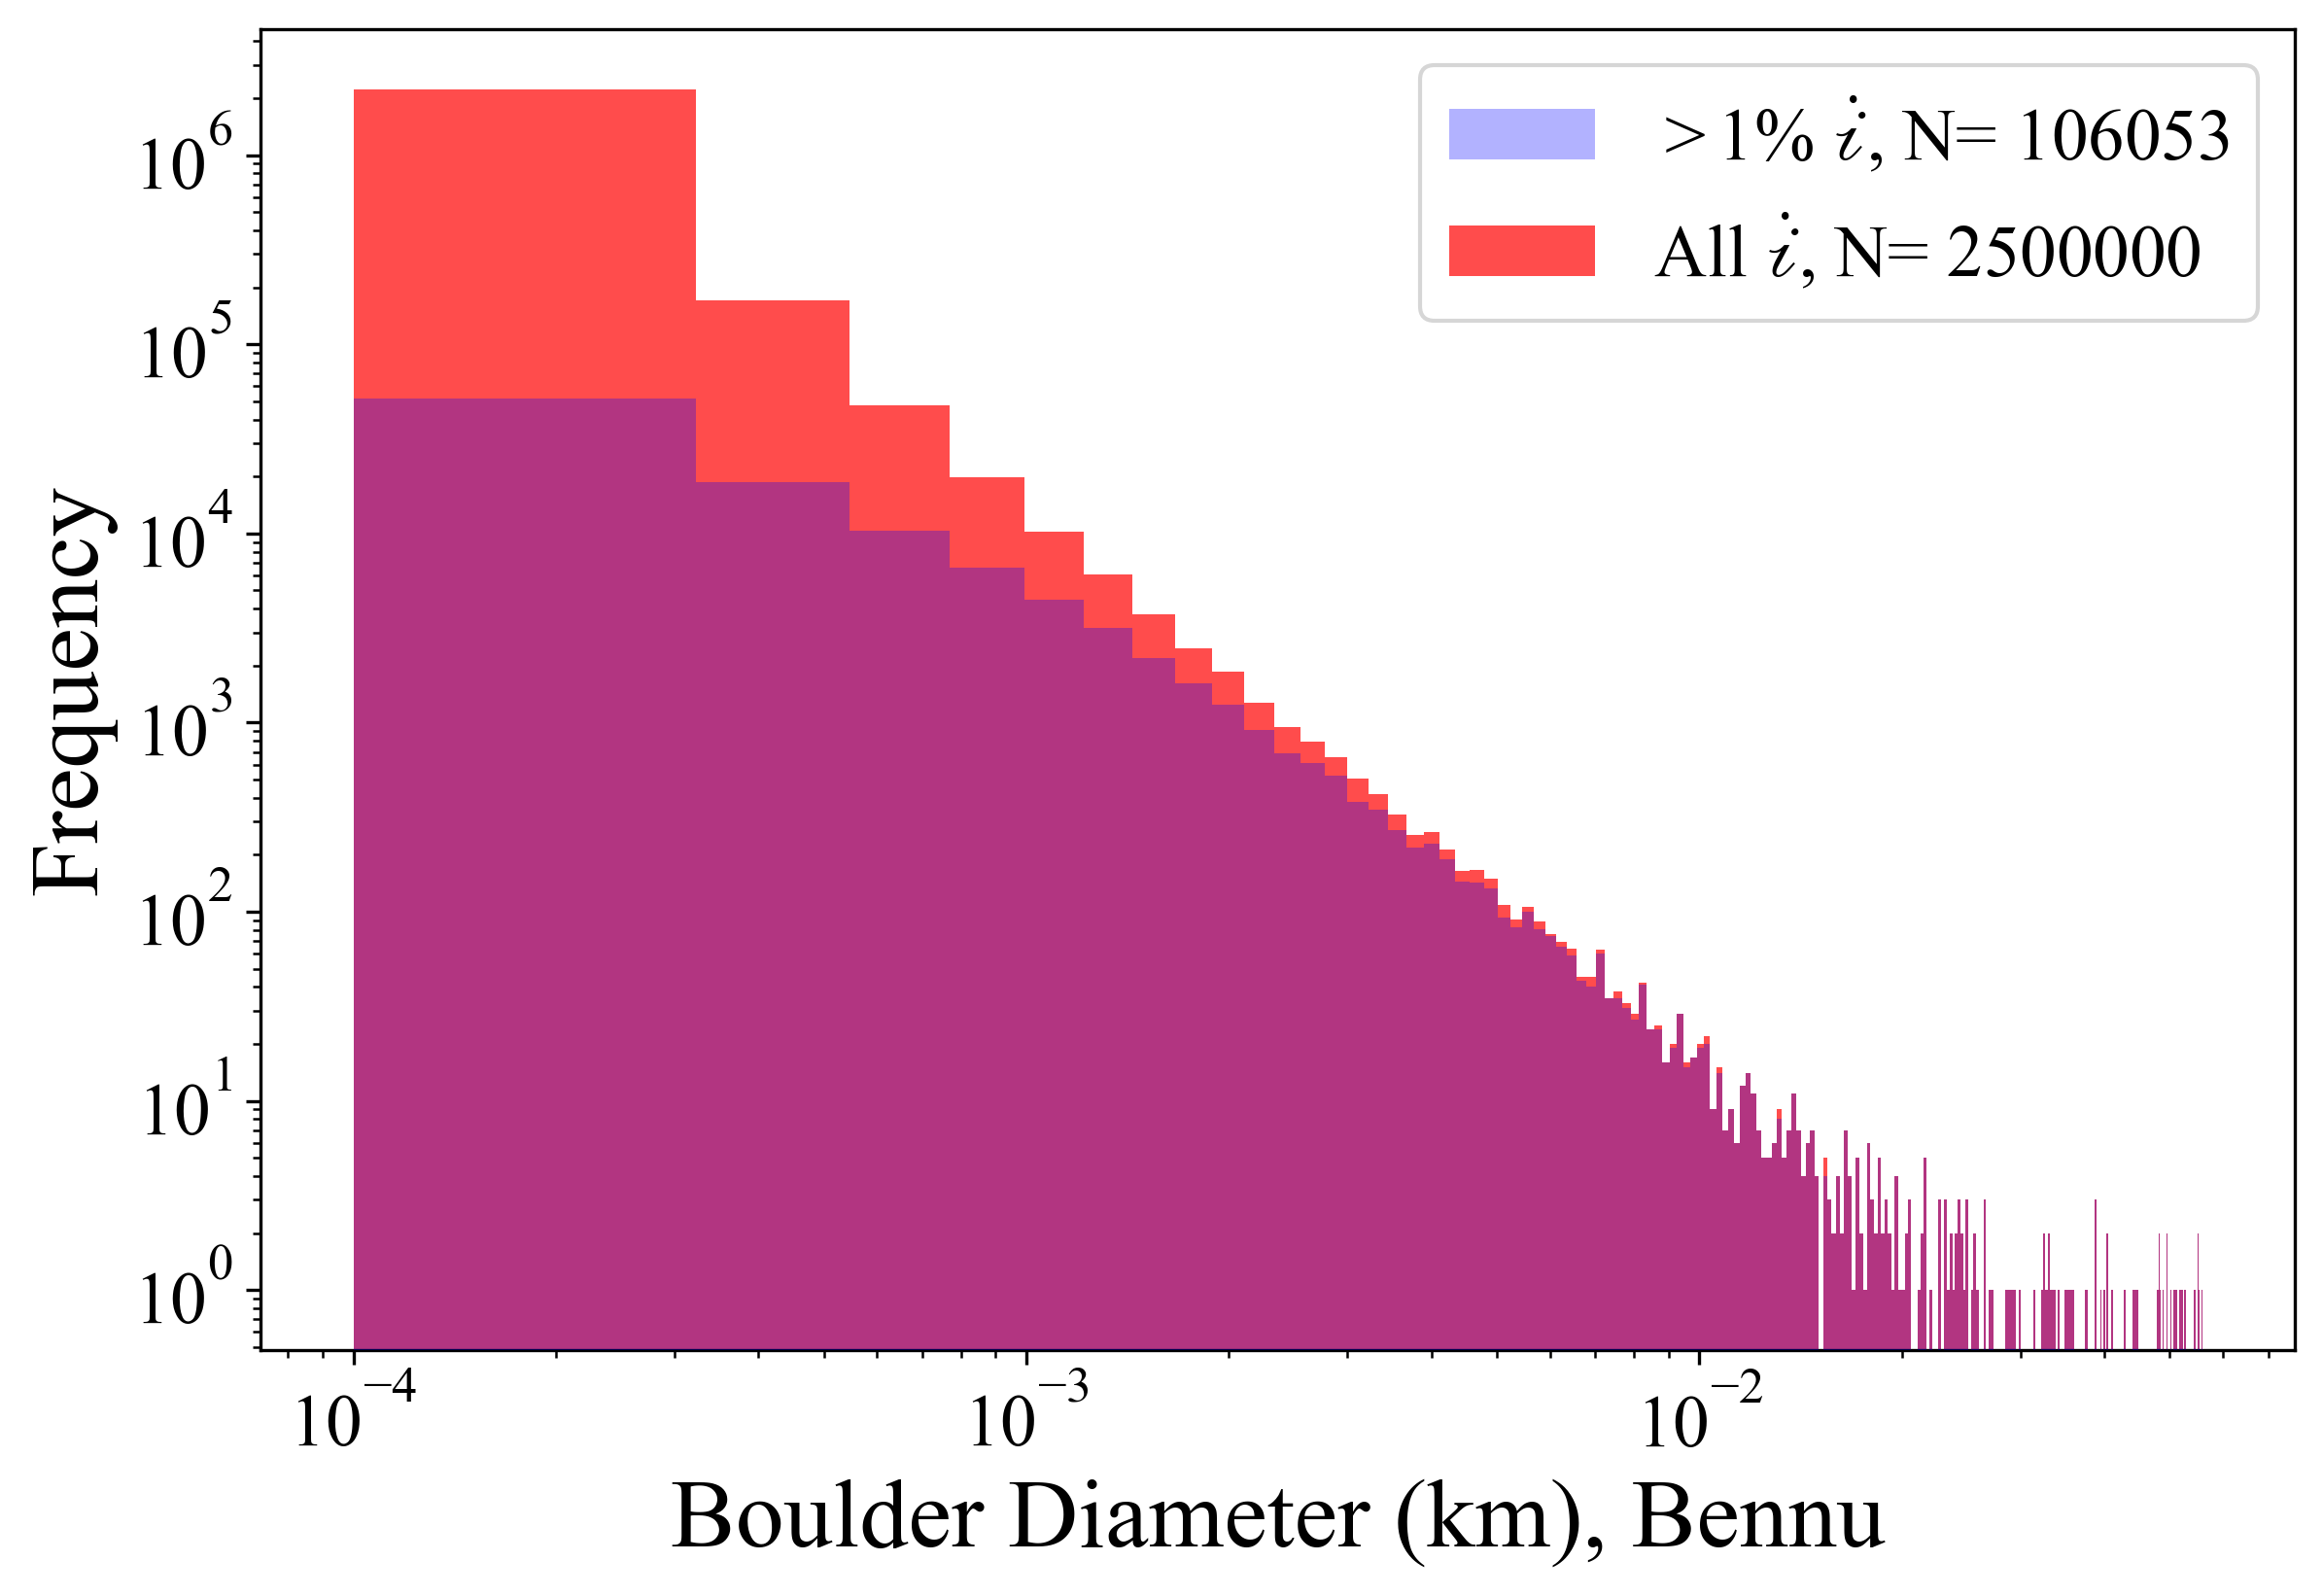
\includegraphics[width=\textwidth]{fig/boulder_sizes_biggerthan1_bennu.png}
        \caption{Bennu's subsampled results of diameter and percent contribution to solar inclination change}
    \end{subfigure}
    \hfill
    \begin{subfigure}{0.49\textwidth}
        \centering
        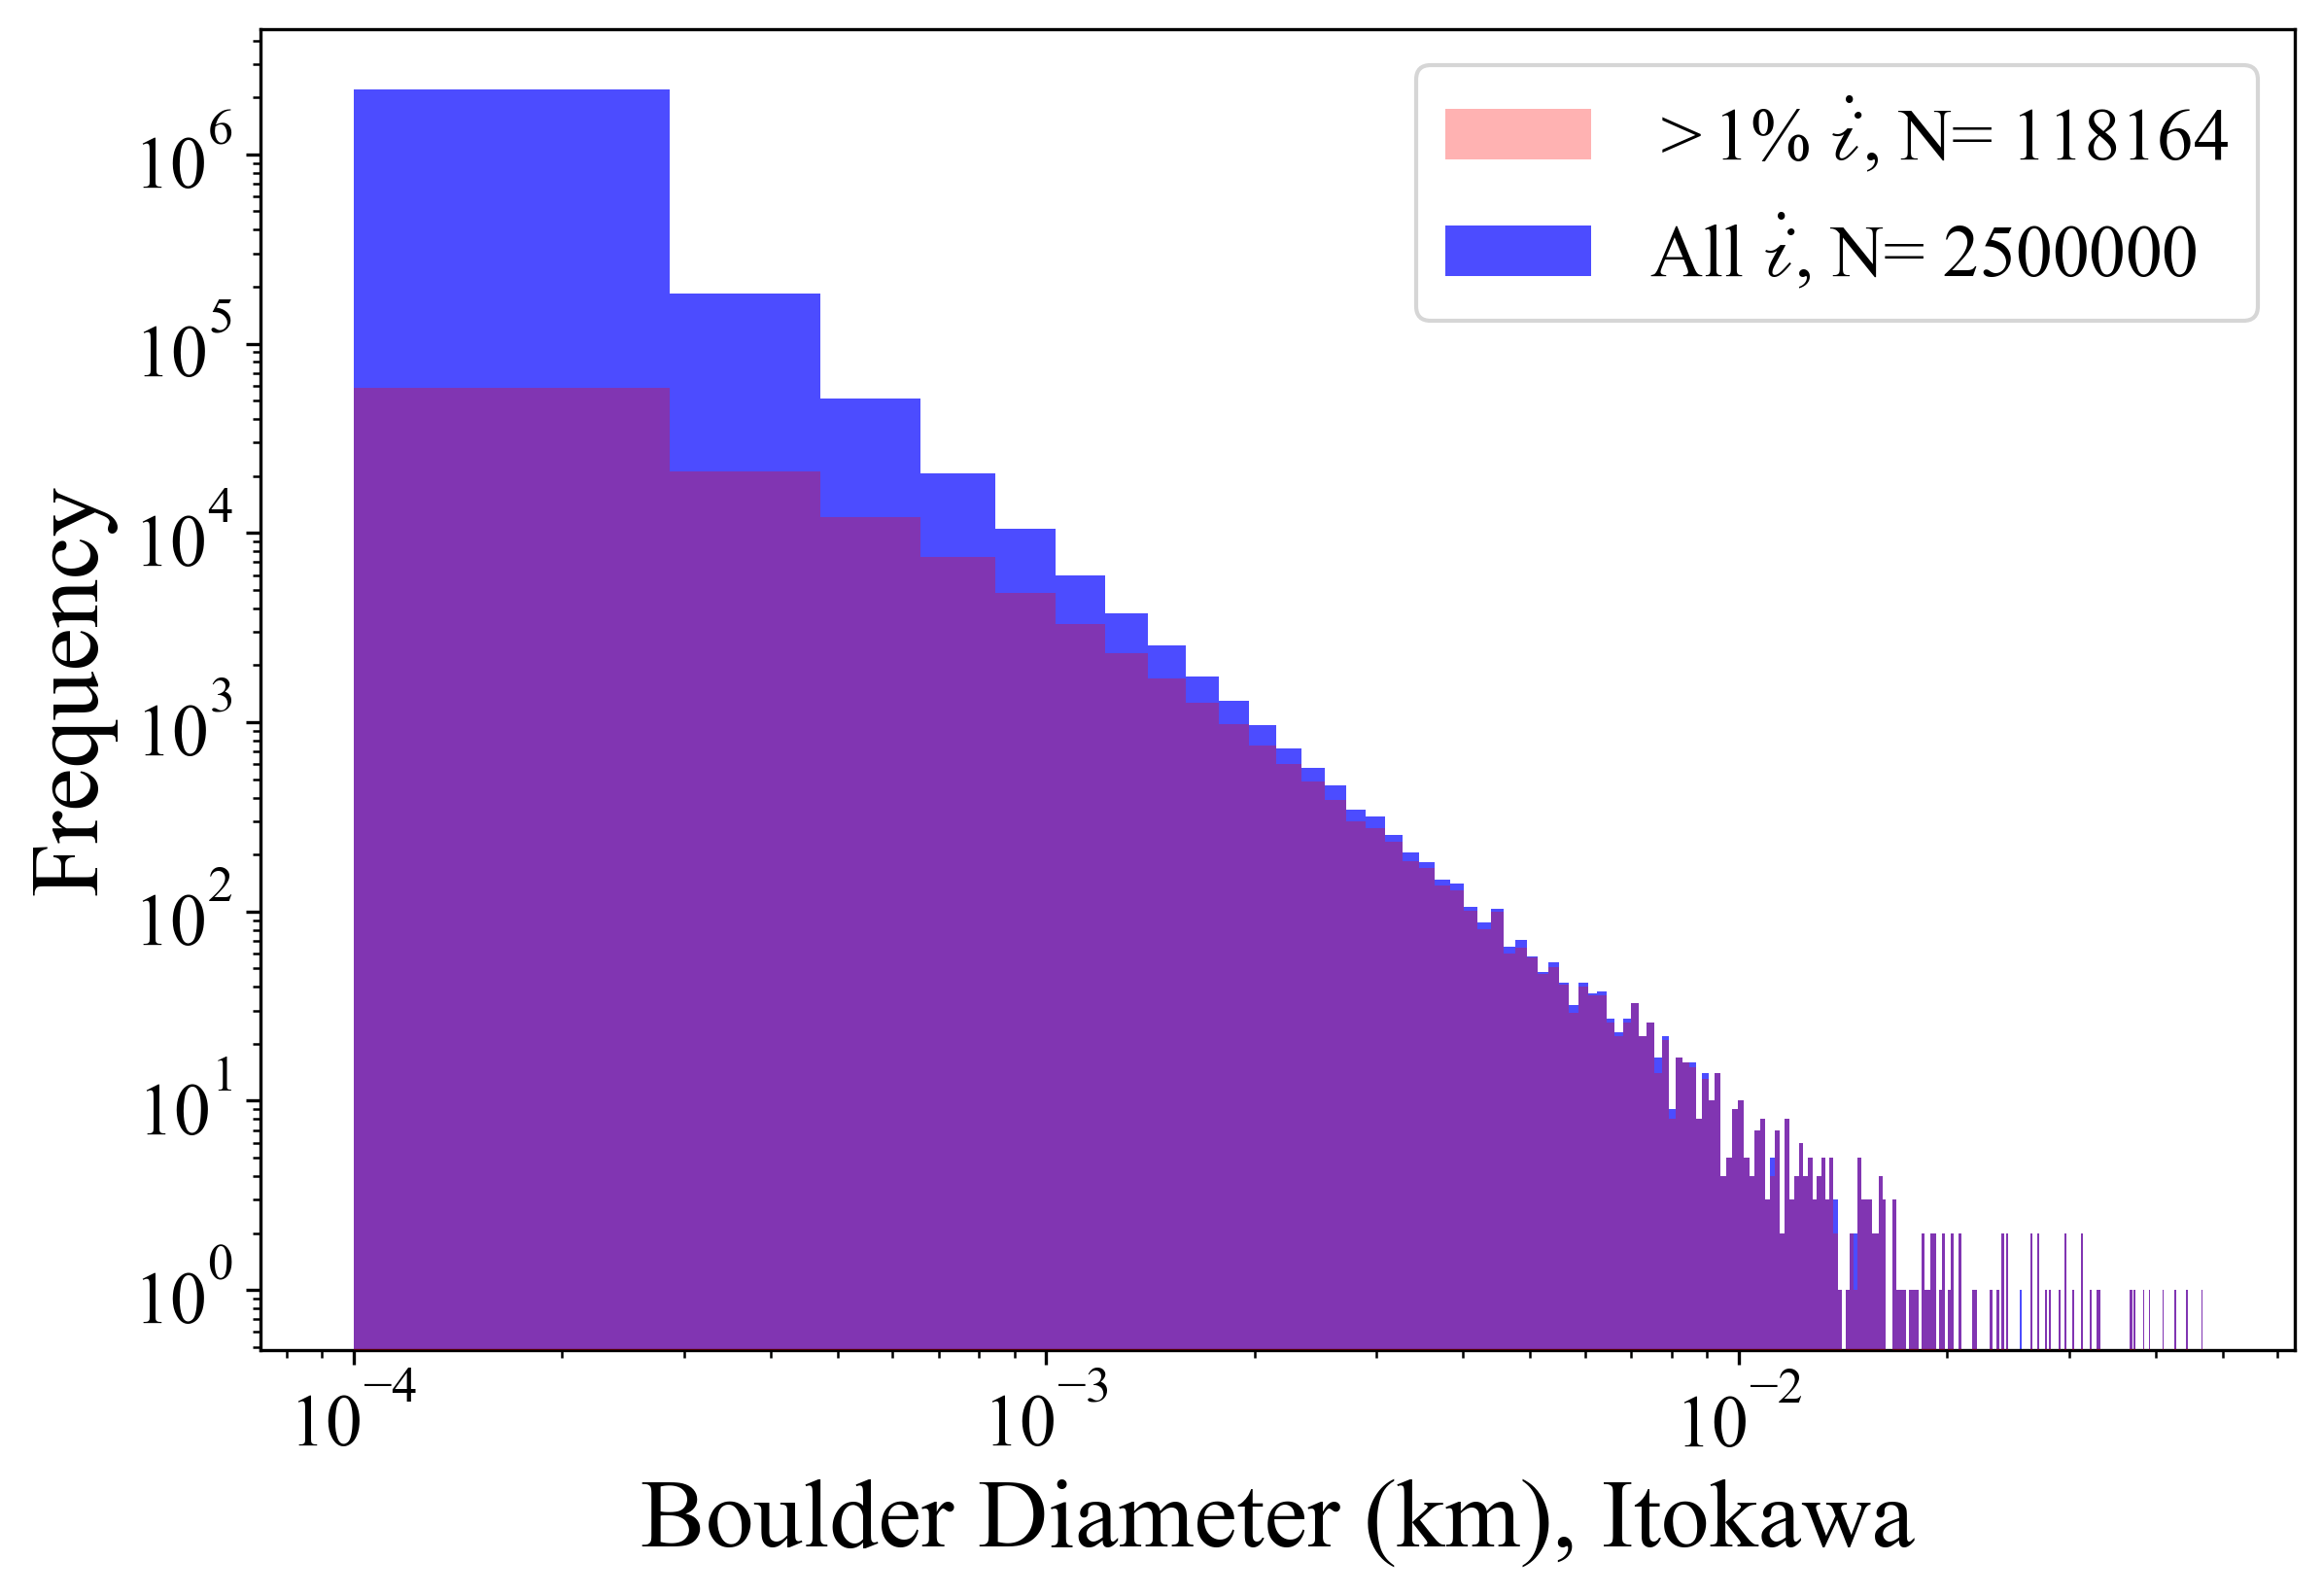
\includegraphics[width=\textwidth]{fig/boulder_sizes_biggerthan1_itokawa.png}
        \caption{Itokawa's subsampled results of diameter and percent contribution to solar inclination change}
    \end{subfigure}  
    \caption{Full histogram of boulder diameters compared to the subsampled set that represents boulders contributing $> 1\%$ to solar inclination change}
    \label{fig:size_onepercent}
\end{figure}

The next factor that was randomized during simulations was the dominant face orientation of the boulder model. Each boulder was modeled by a wedge prism with a $90^{\circ}$ angle, leaving one face to be the largest and projecting the dominant force for the shape. When binning boulders by their percent contribution to overall YORP, we see a trend arise with increasing YORP inclination change influence. The lightest color in Fig. \ref{fig:west_onepercent} is the population contributing less than $0.1\%$ to overall YORP. Each darker shade represents a 10x increase in the percentage bound. What is seen with this increase is a departure of boulders near $\pi/2$ and $3\pi/2$, which represents directly North and South facing dominant boulders. This is subtle and only represents a $5\%$ bias towards east and west facing boulders. There is a much larger bias when examining the difference in the angular acceleration terms. %We would expect to see that west and east facing boulders influence obliquity at a higher percentage when obliquities are still low. 

\begin{figure}[H]
    \begin{subfigure}{0.49\textwidth}
        \centering
        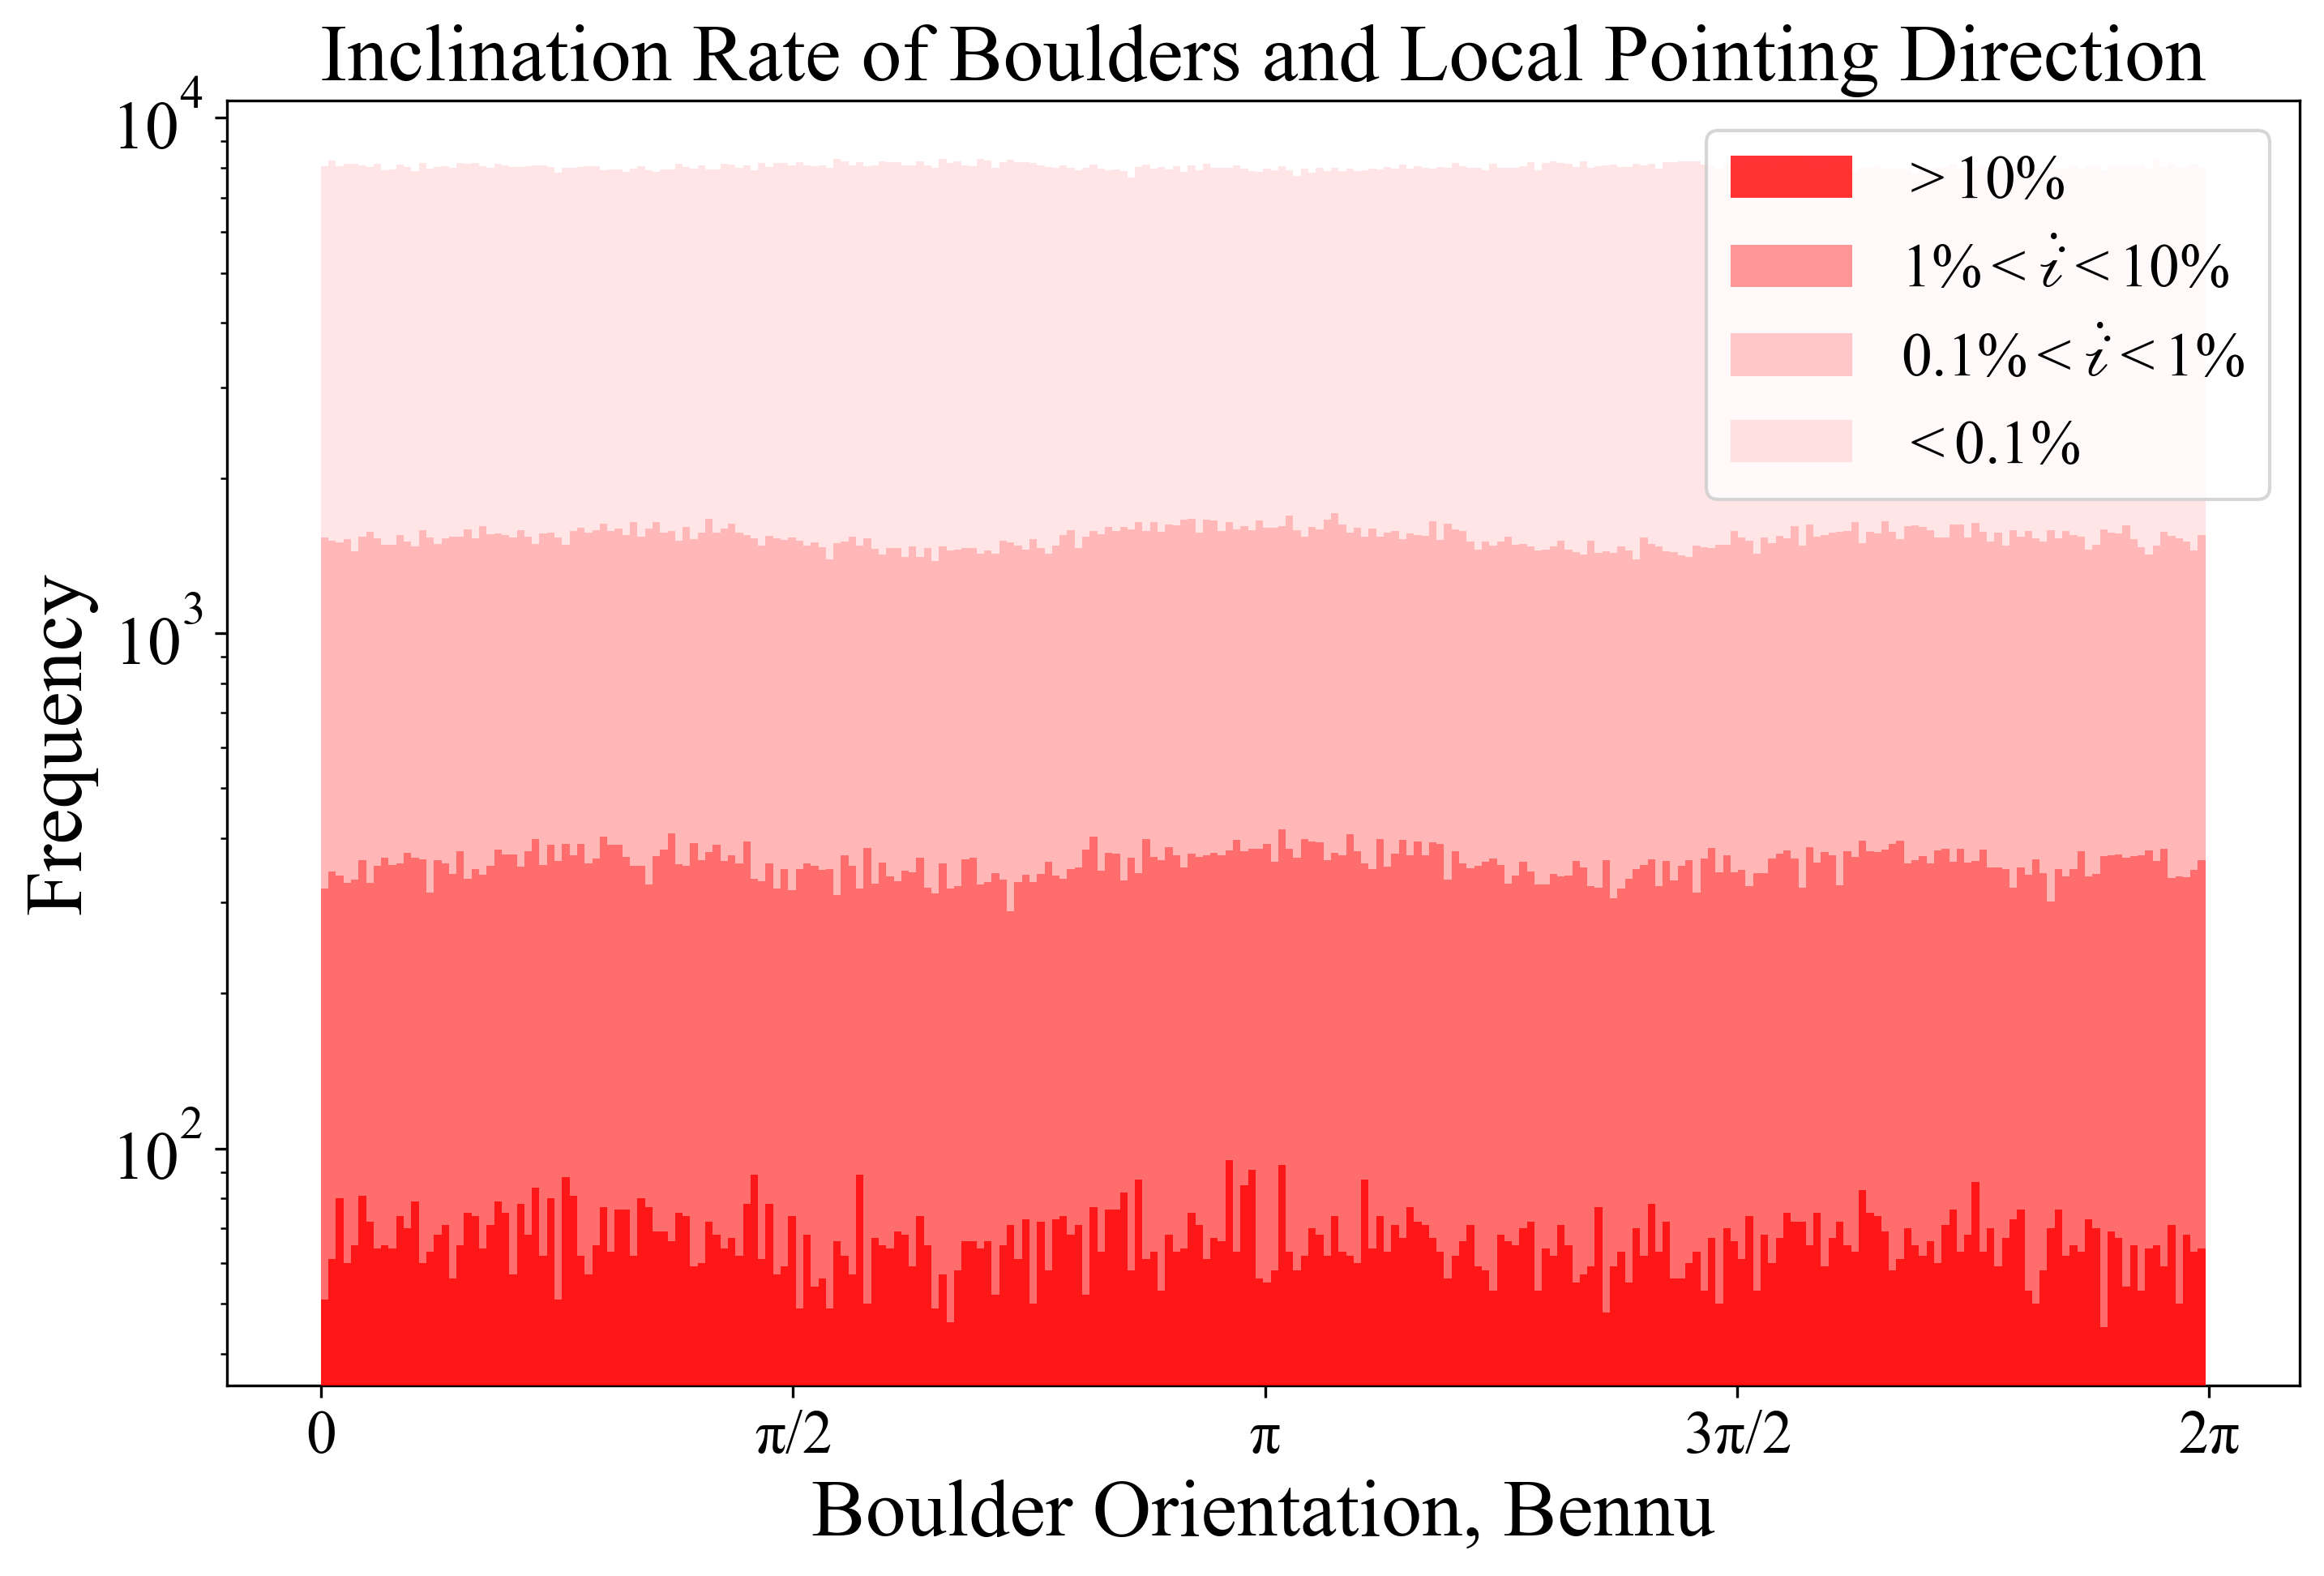
\includegraphics[width=\textwidth]{fig/boulder_west_stacked_bennu.png}
        \caption{Bennu's orientation pointing distribution separated by percent contribution to global solar inclination change rate}
    \end{subfigure}
    \hfill
    \begin{subfigure}{0.49\textwidth}
        \centering
        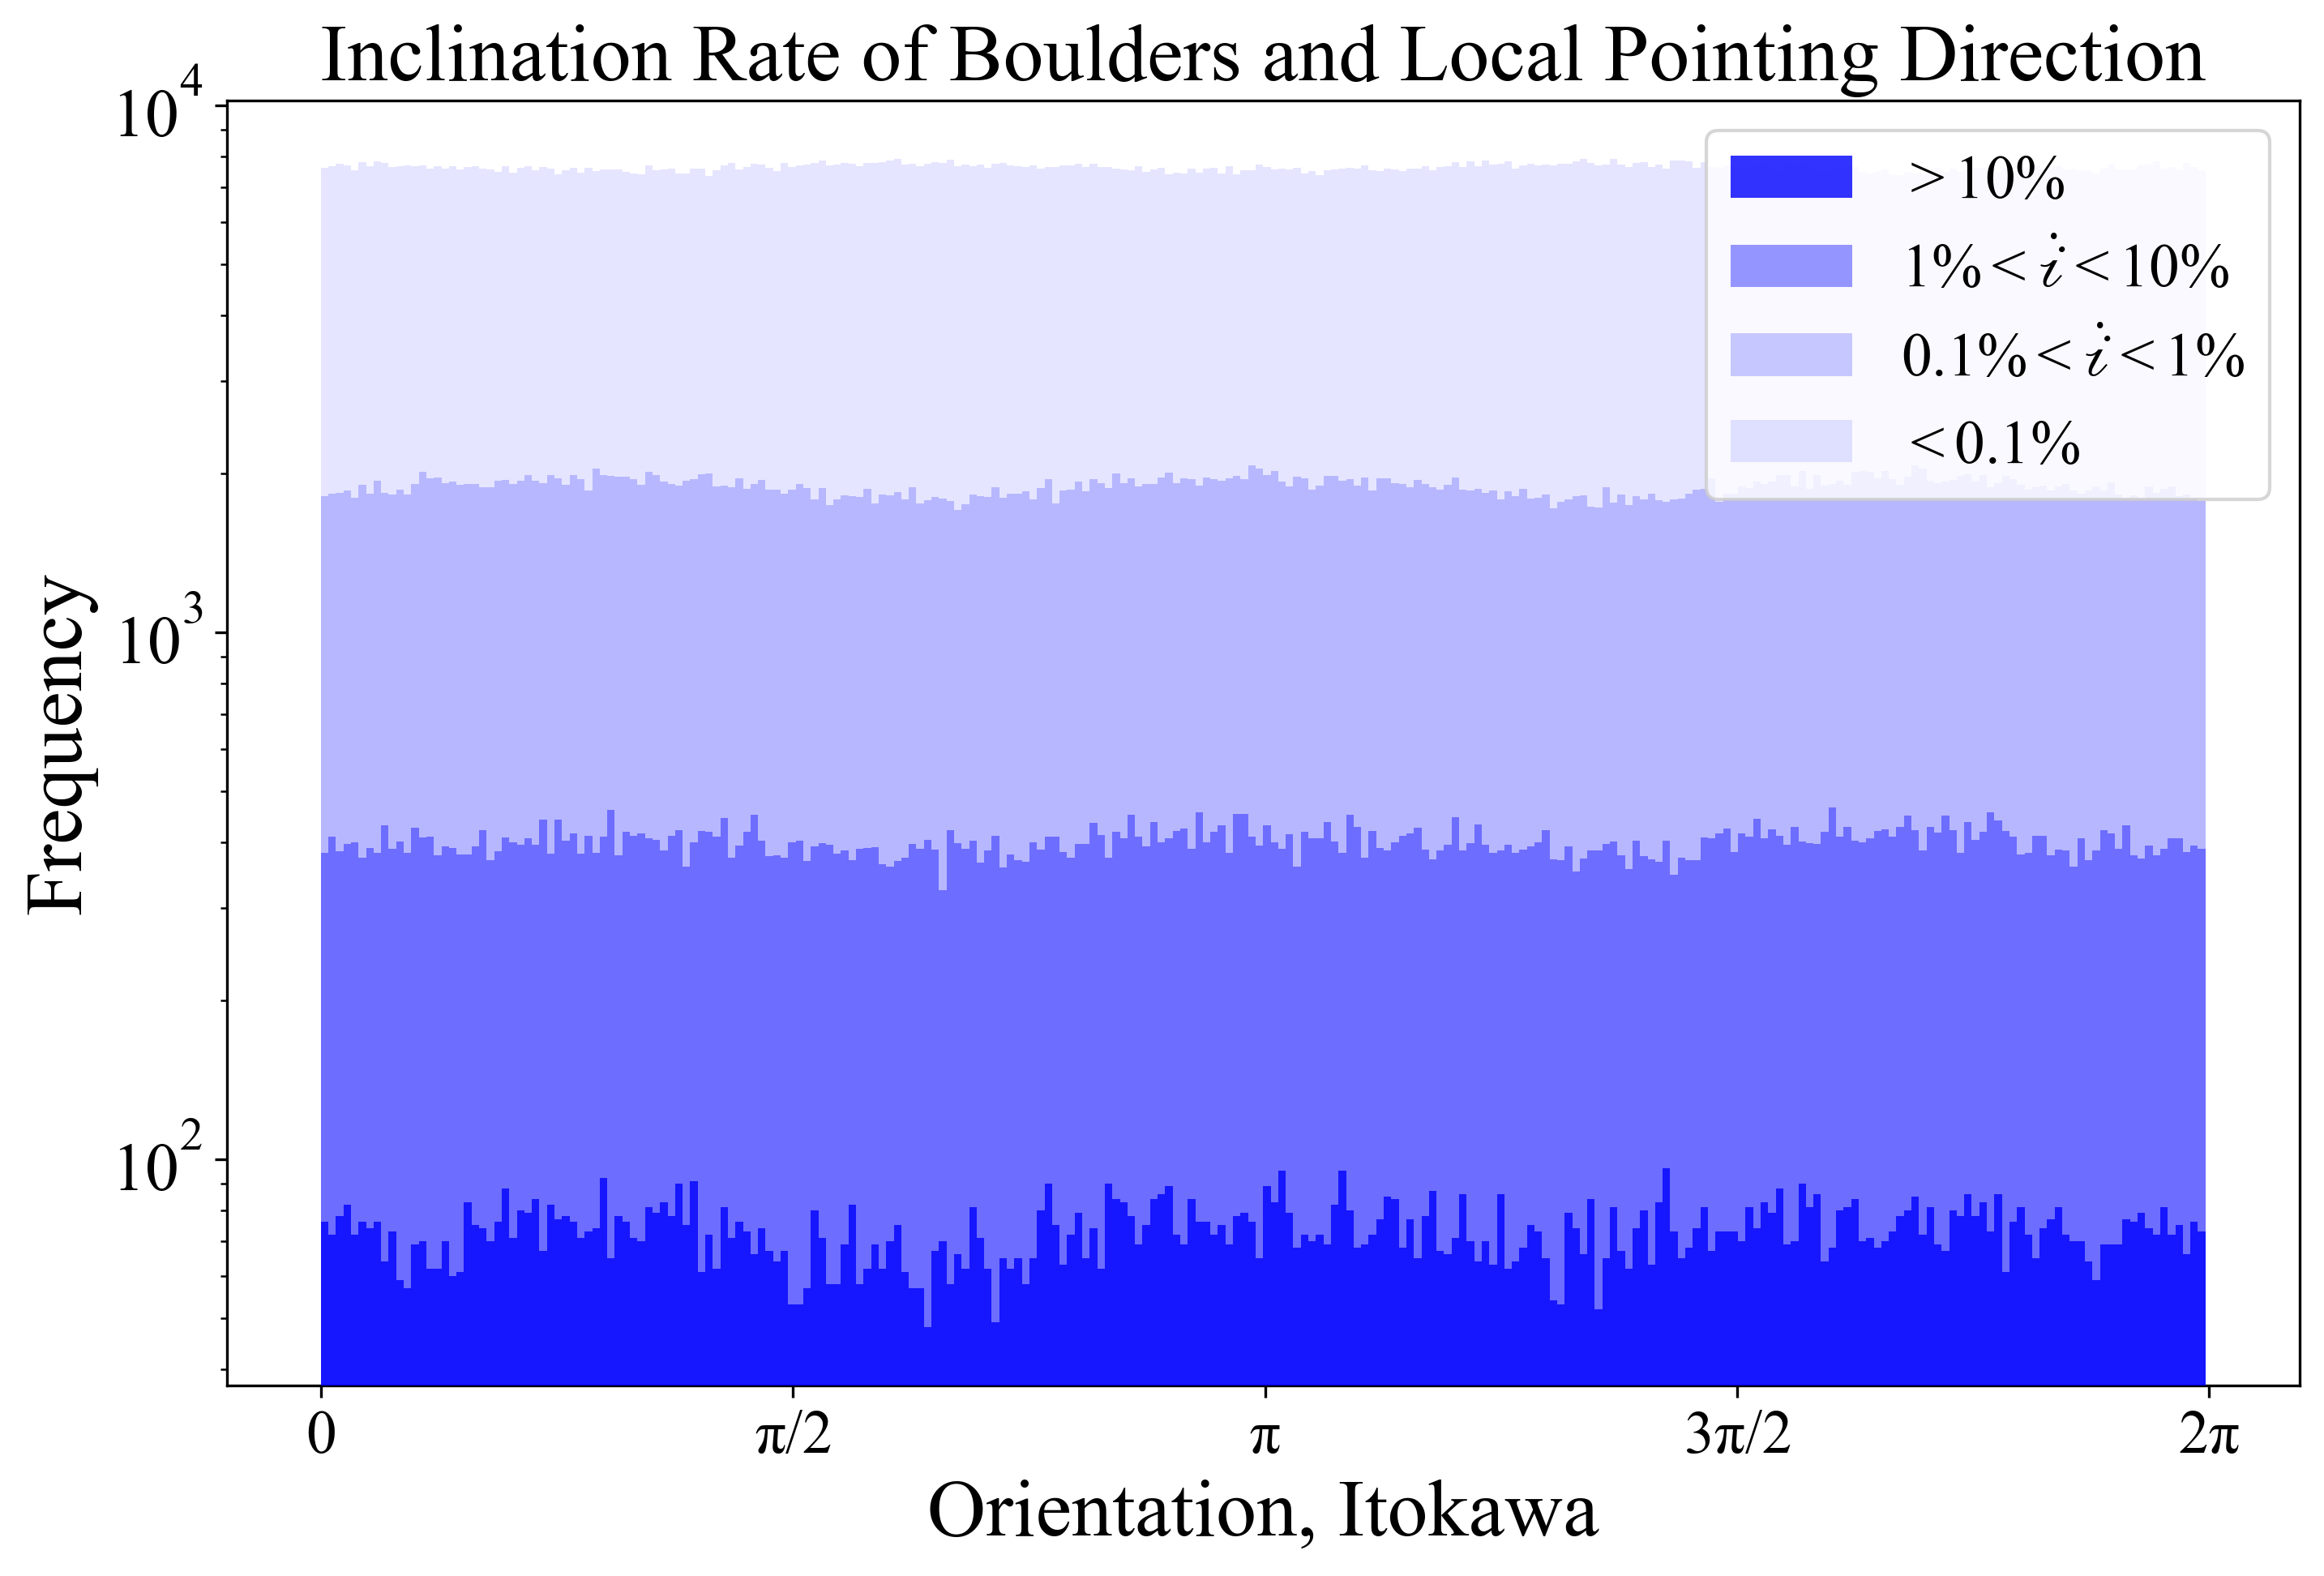
\includegraphics[width=\textwidth]{fig/boulder_west_stacked_itokawa.png}
        \caption{Itokawa's orientation pointing distribution separated by percent contribution to global solar inclination change rate}
    \end{subfigure}  
    \caption{Varying bins of percent contribution to solar inclination change, with darker colors representing higher \% change from a single boulder, distributed over dominant pointing direction}
    \label{fig:west_onepercent}
\end{figure}

Lastly we examine the longitude and latitude biases for large contributing boulders. As YORP torque strength is proportional to the norm of the vector from the body center of mass to the surface location of the boulder, we would expect to see larger contributing boulders in areas with high magnitude $|\vec{r}|$. An interesting result from this sensitivity analysis is that we see less influential boulders near the equators when filtering by inclination or obliquity rates. This is shown for both Bennu and Itokawa shapes, see Fig. \ref{fig:location_percents}. This is the opposite trend from large spin contributing boulders. This can be explained by the difference in spin-inducing YORP factors and obliquity-inducing YORP factors. When a boulder contributes a large value to YORP obliquity, it must induce asymmetry in the xy-plane. Therefore, the boulders located at the equator that contribute equally to torque in the northern and southern hemispheres cause a net close-to-zero solar inclination change.

\begin{figure}[H]
    \begin{subfigure}{0.49\textwidth}
        \centering
        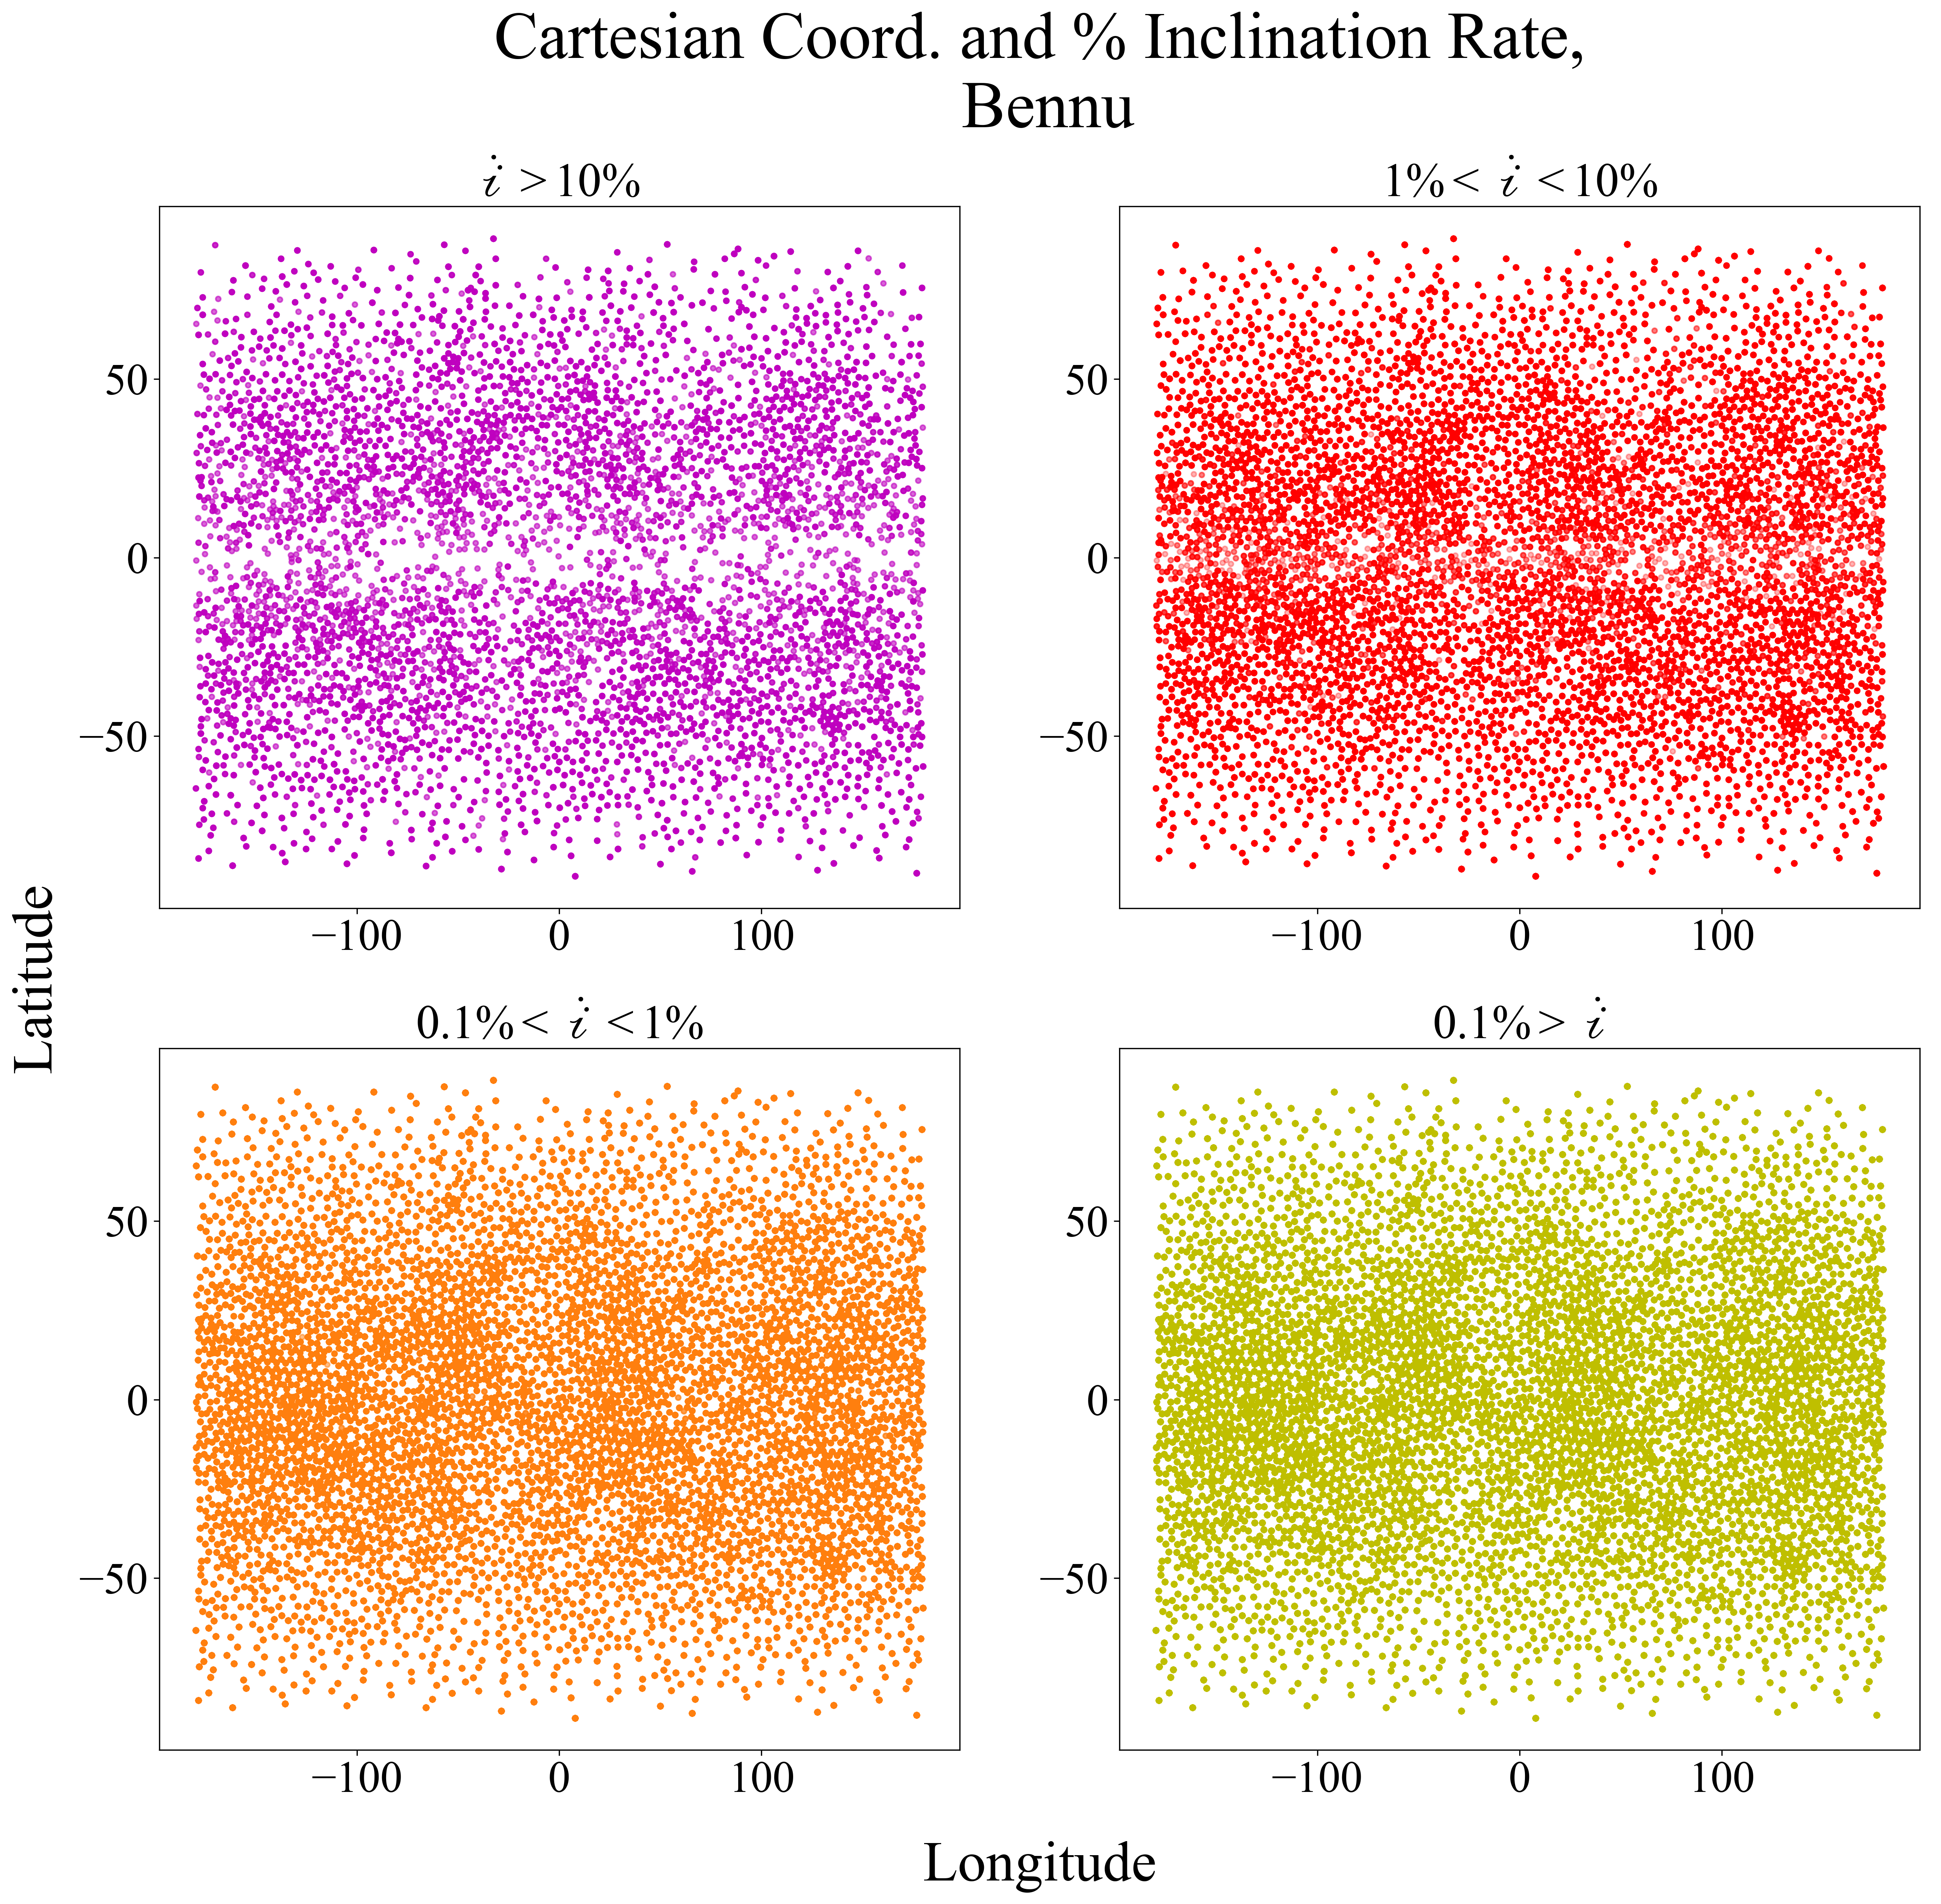
\includegraphics[width=\textwidth]{fig/location_dists_bennu.png}
        \caption{Bennu location distribution separated into contributing levels to solar inclination change}
    \end{subfigure}
    \hfill
    \begin{subfigure}{0.49\textwidth}
        \centering
        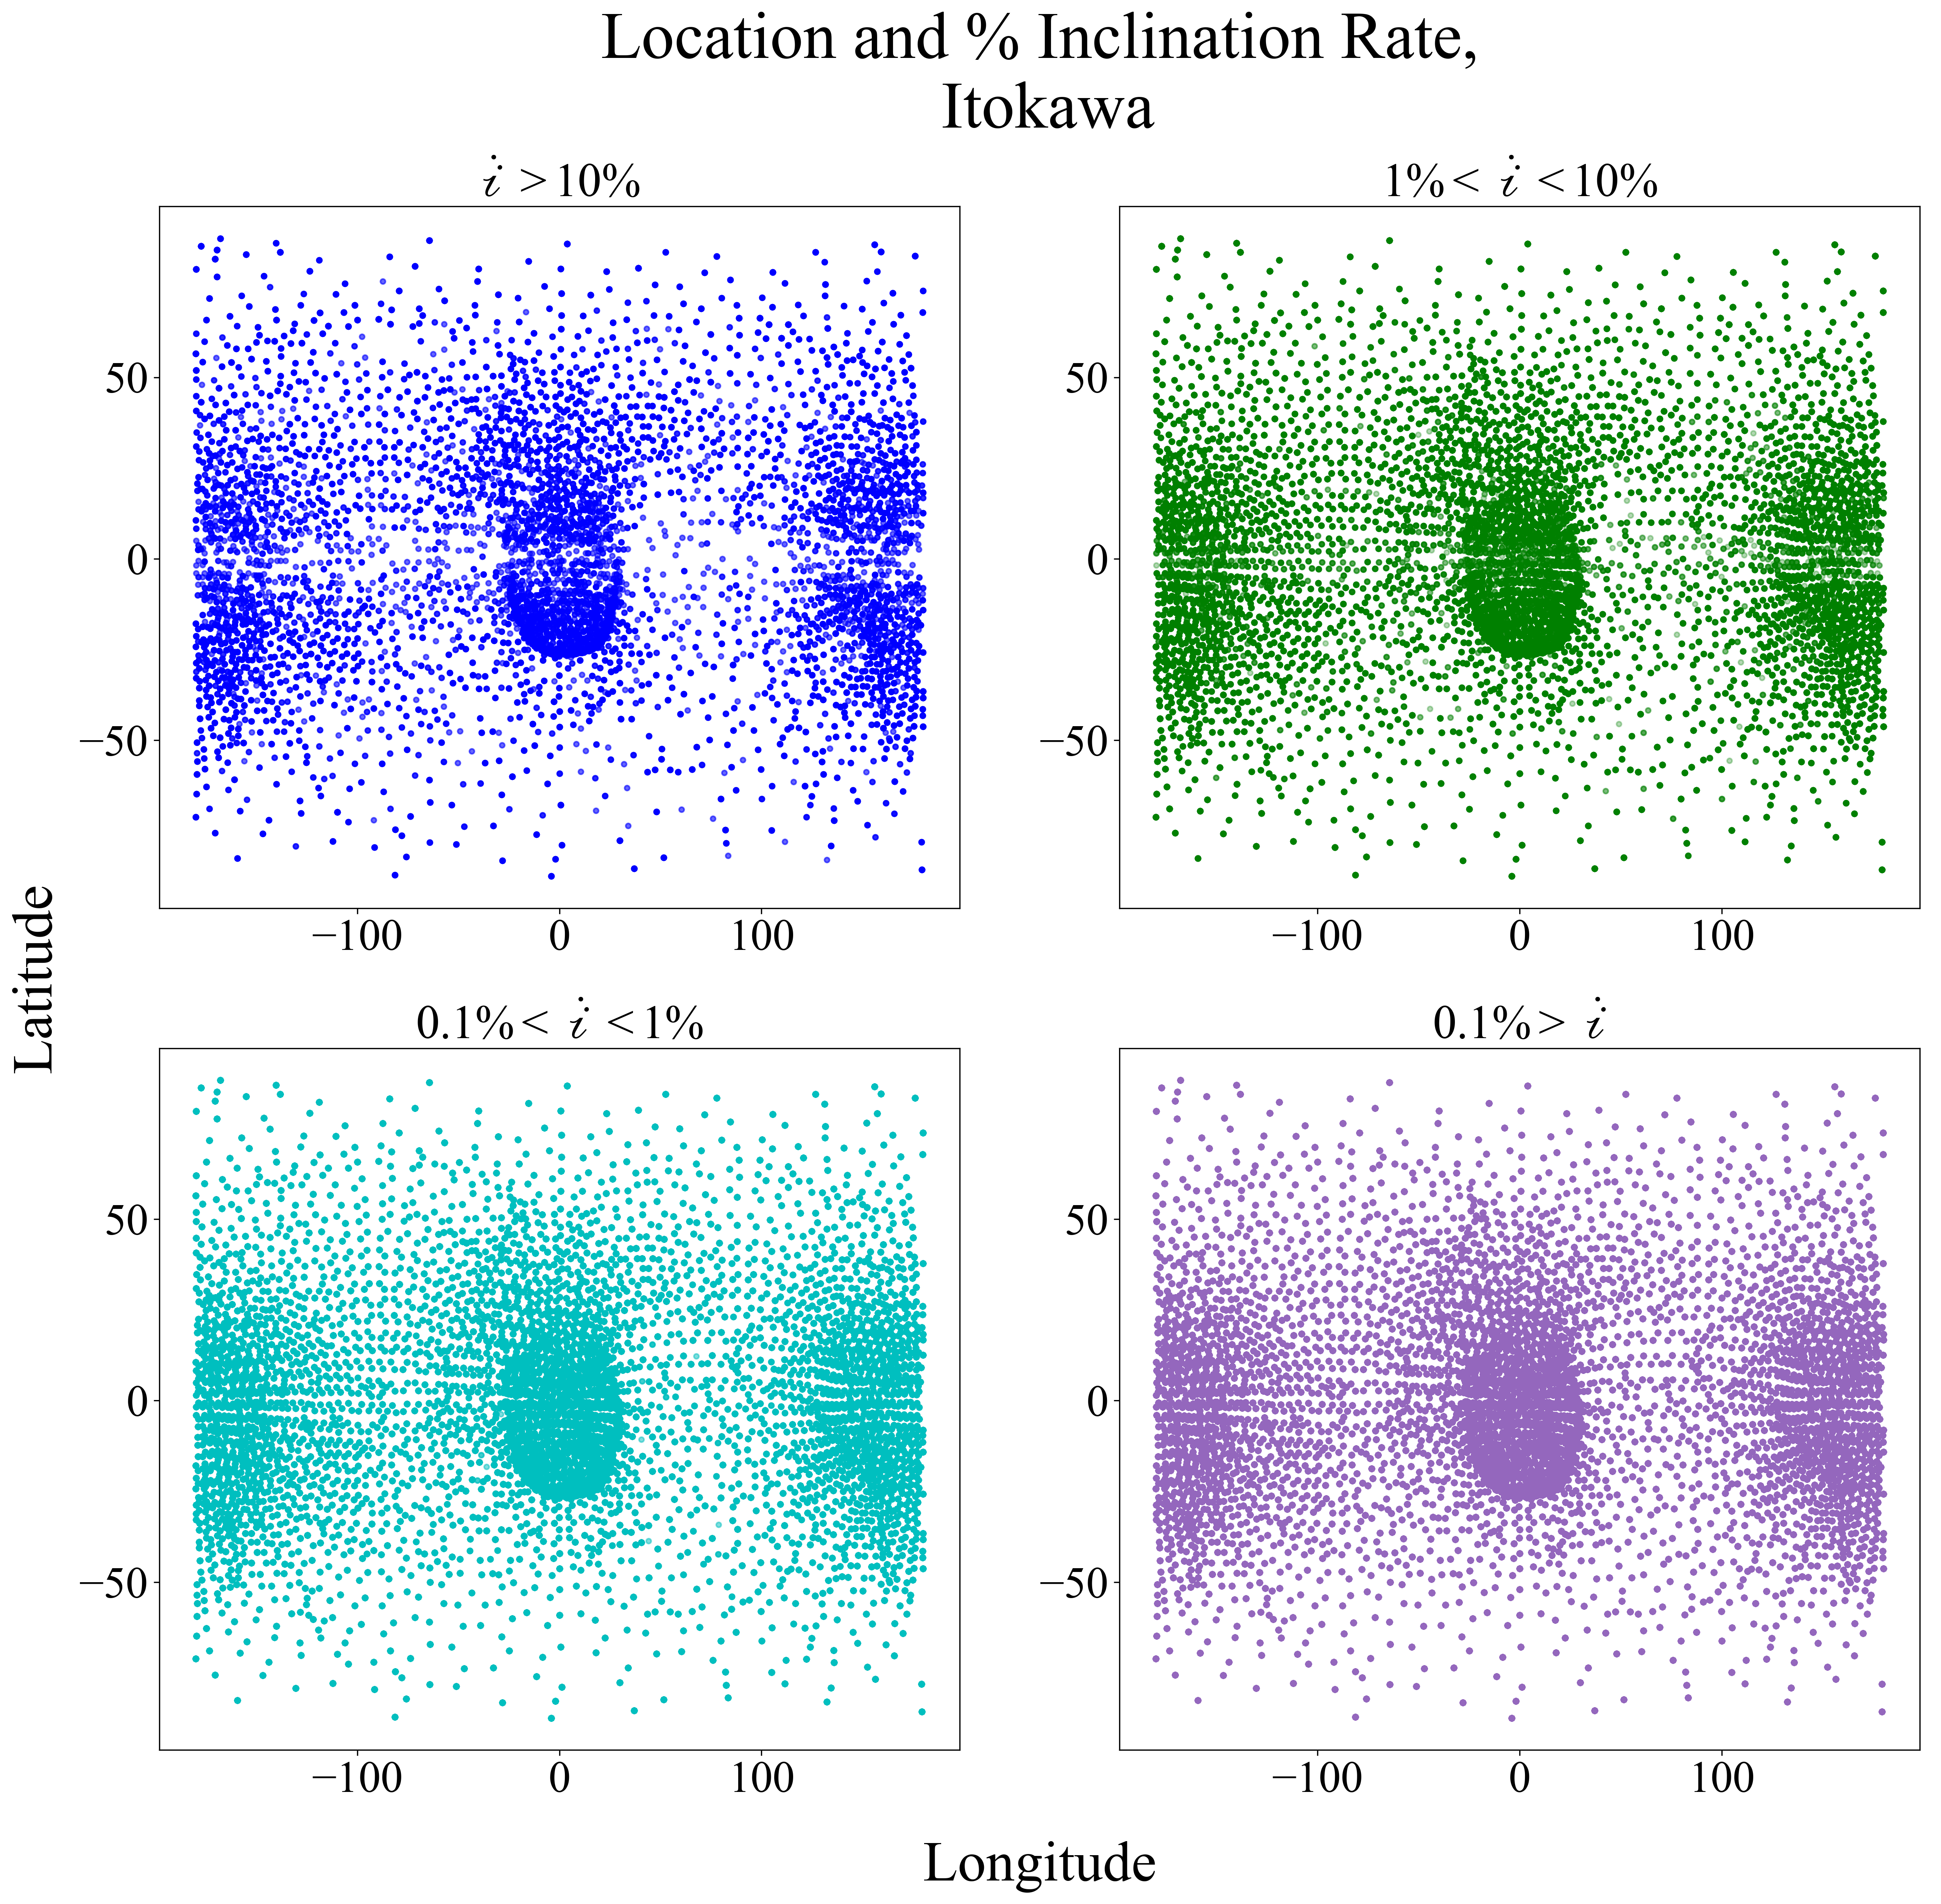
\includegraphics[width=\textwidth]{fig/location_dists_itokawa.png}
        \caption{Itokawa location distribution separated into contributing levels to solar inclination change}
    \end{subfigure}  
    \caption{Boulder locations separated by percent contribution, showing a departure of boulders from equator at rates of > 1\% and > 10\% for both bodies}
    \label{fig:location_percents}
\end{figure}

These results tell us about the influential factors that make an asteroid overall YORP obliquity rate estimate sensitive to boulder presence. This applies the statistics provided from observation and translates them into dynamical predictions. The range of $\dot{\mathit{i}}_s$ shown here is the possible variation in obliquity due to randomized boulders. Any of our current YORP estimates may fall into this range if boulders are mismodeled or unmodeled.



%\subsection{Pole Stability}

%Now we measure the pole stability over time as we propagate an average case with boulders. We will show pole evolution, identify when the tumbling criterion are met, and also show how often or easily we can drive the spin state to disaggregation as it is defined in Scheeres and Sanchez equation for velocity of cohesion loss (find actual name of this)

%%%%%%%%%%%
%%%%%%%%%%%
%%%%%%%%%%%%%% ANALYSIS NEEDED %%%%%%%%%%%%%%%%%%%%%%%%%%%%%%%%%%%%%%%%%%%%%%%%%%
%%%%%%%%%%%
%%%%%%%%%%%

\subsection{Boulder Motion}
We compare boulder YORP contributions at different locations to make inferences about the impact of boulder's moving on the body's surface. This behavior has been discussed previously and explains the presence of features such as infilled craters on asteroids \citep{Brack2019}. In Fig. \ref{fig:ob_motion_nodelta}, we sample boulders within $5^{\circ}$ of longitude and up to $9.43^{\circ}$ in latitude apart. Their obliquity rate contributions, shown as $\dot{i}_s$, follow a distinct linear relationship with latitude. Note that we report in rad/day rather than seconds in order to contextualize boulder motion on a more realistic timescale.
\begin{figure}[H]
    \centering
    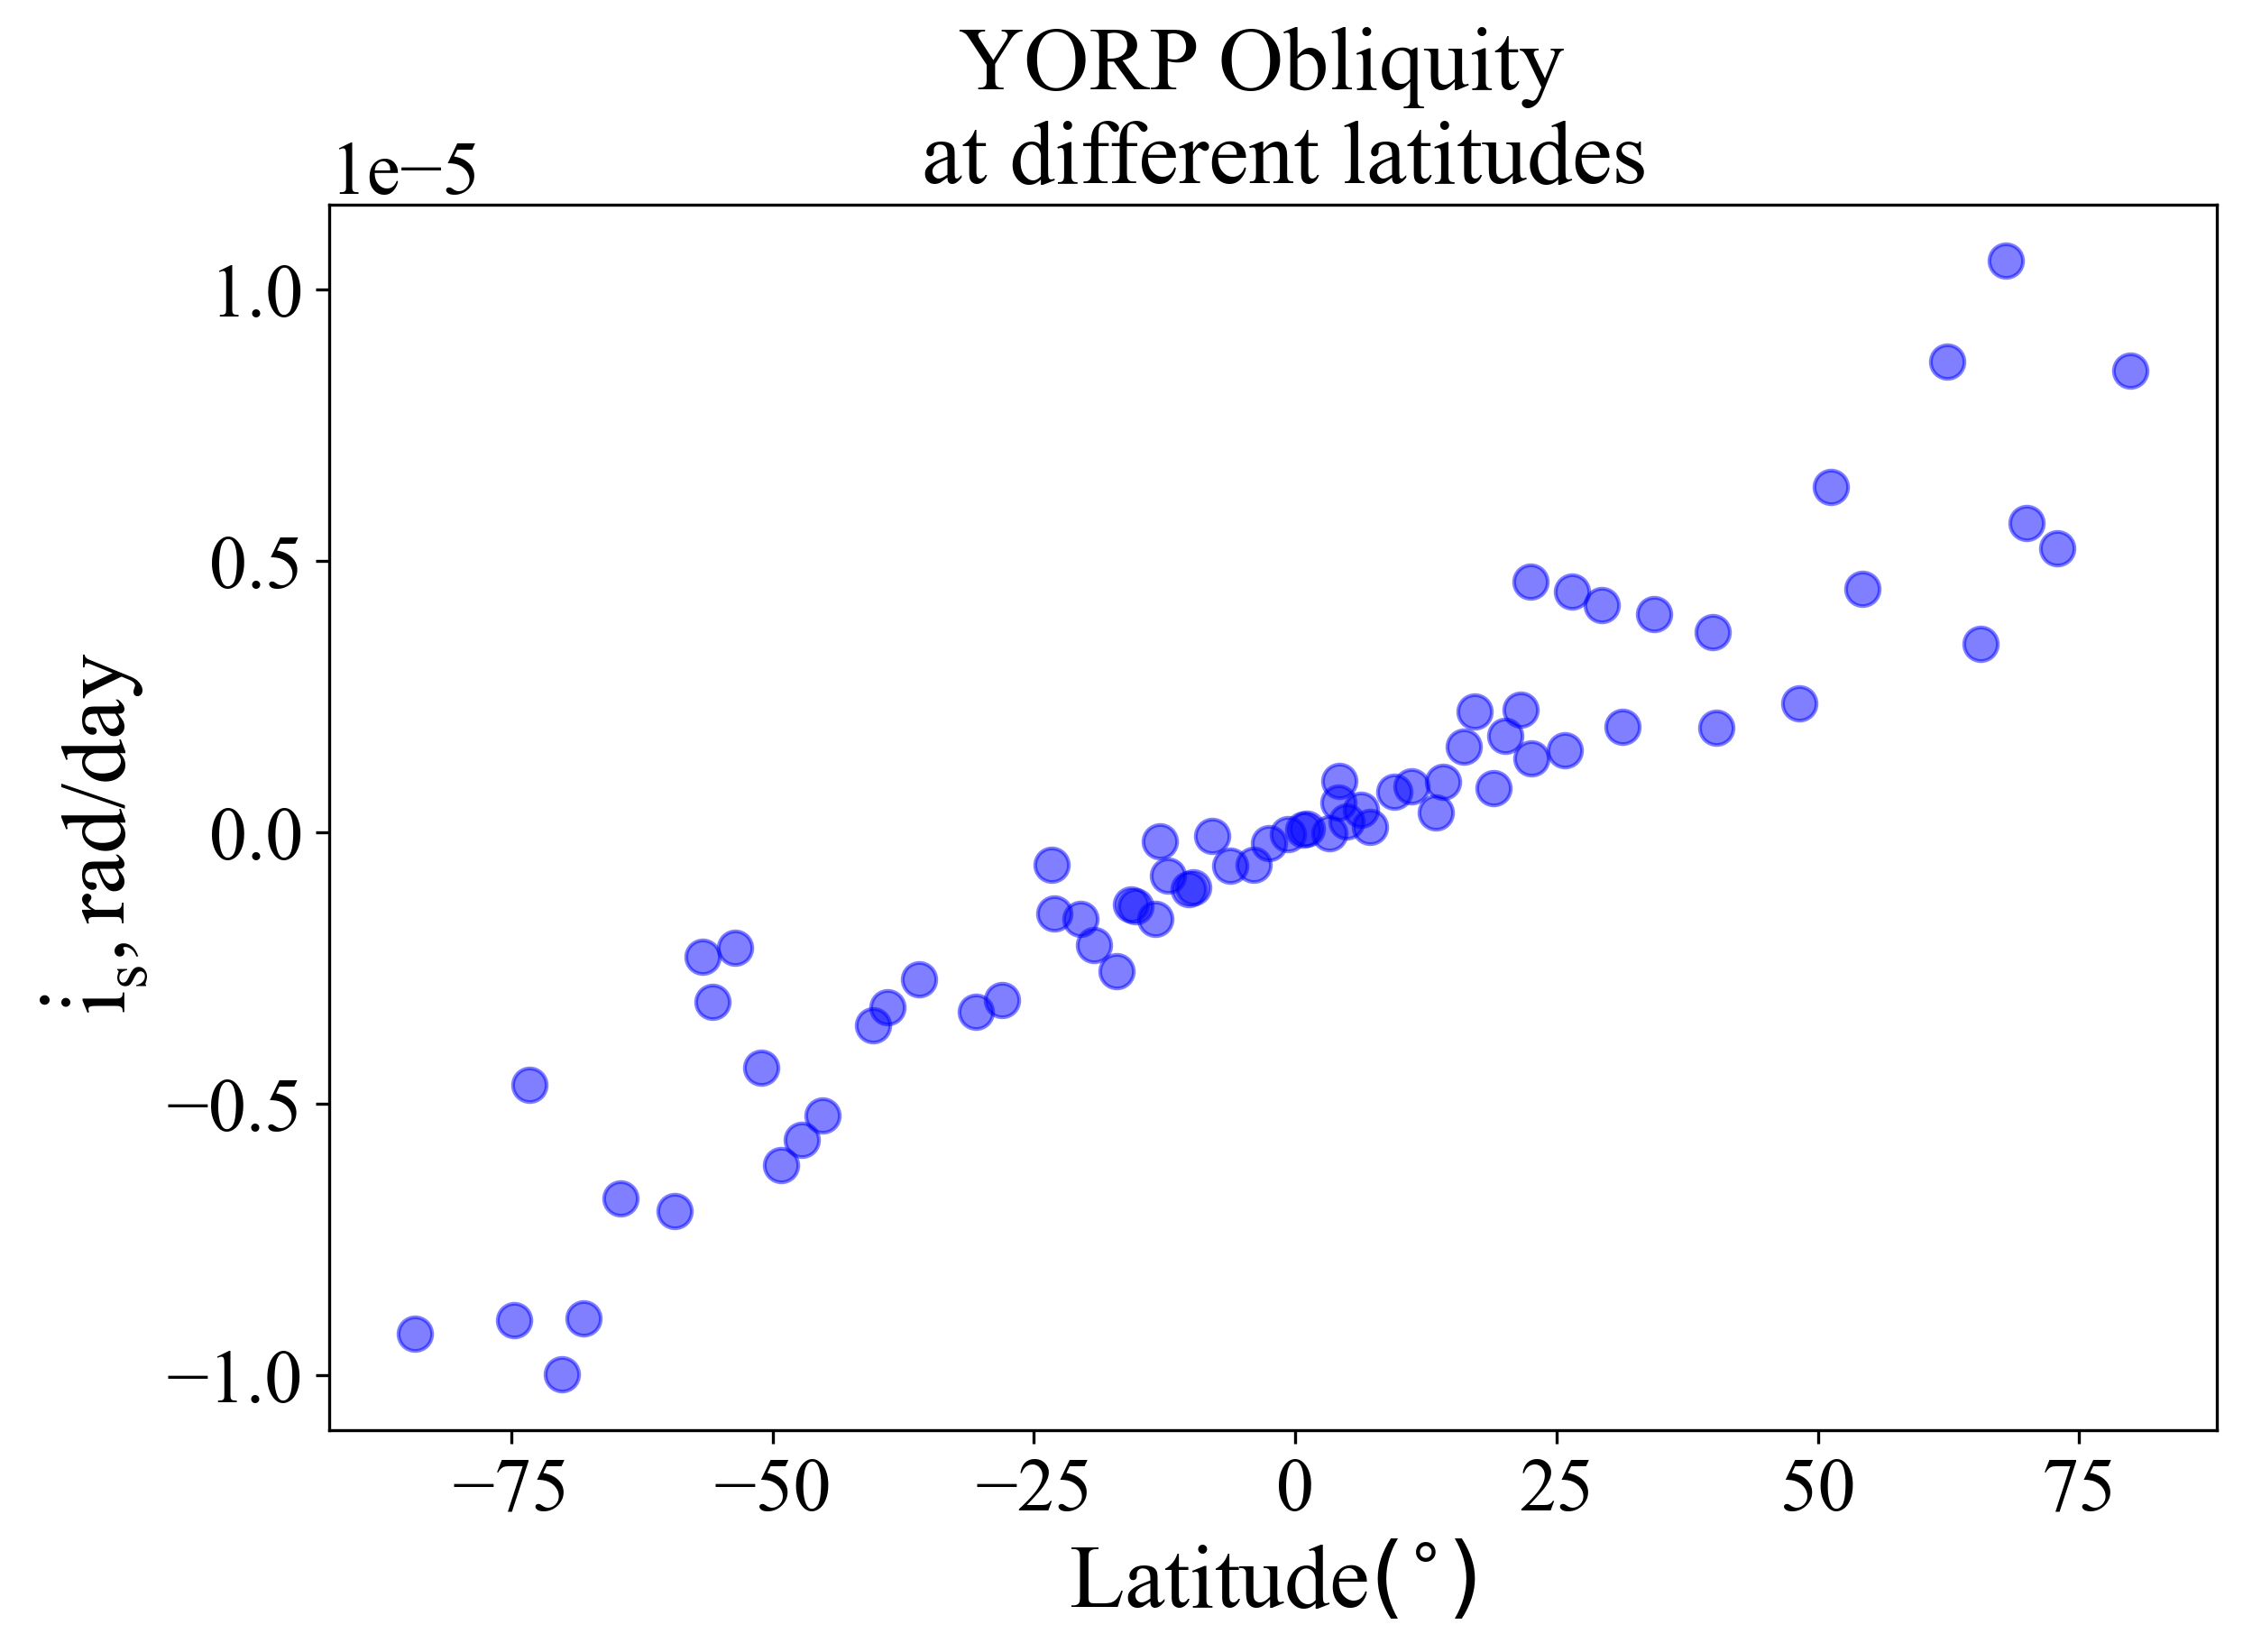
\includegraphics[width=0.5\textwidth]{fig/obliq_amt_boulder_motion_bennu.png}
    \caption{Differing amounts of YORP obliquity acceleration for boulders within 5 degrees in longitude but varying latitudes}
    \label{fig:ob_motion_nodelta}
\end{figure}

Comparing the differences between neighboring boulders gives a more random relationship. It is shown that a boulder at a higher latitude could have a lower or higher amount of torque changing the body's obliquity. The largest change in $\dot{i}_s$ is $7.06\times 10^{-6} rad/day$. If we saw this increase in obliquity torque from the most influential boulder in this test case, the single boulder alone could cause a spin pole tilt rate exceeding even the asteroid spin rate within 5 million years. This is one way of describing tumbling behavior and these numbers show how boulders could be the cause of such instability.
This assumes uniform spin is independent of obliquity angle change and we are only looking at dynamics due to a single boulder moving to a highly influential location. The calculations here serve to highlight the magnitude of change due to moving boulders on the surface. In future work, it will be highlighted how necessary it is to simulate boulders moving positions in time as the dynamics change due to YORP.
\begin{figure}[H]
    \centering
    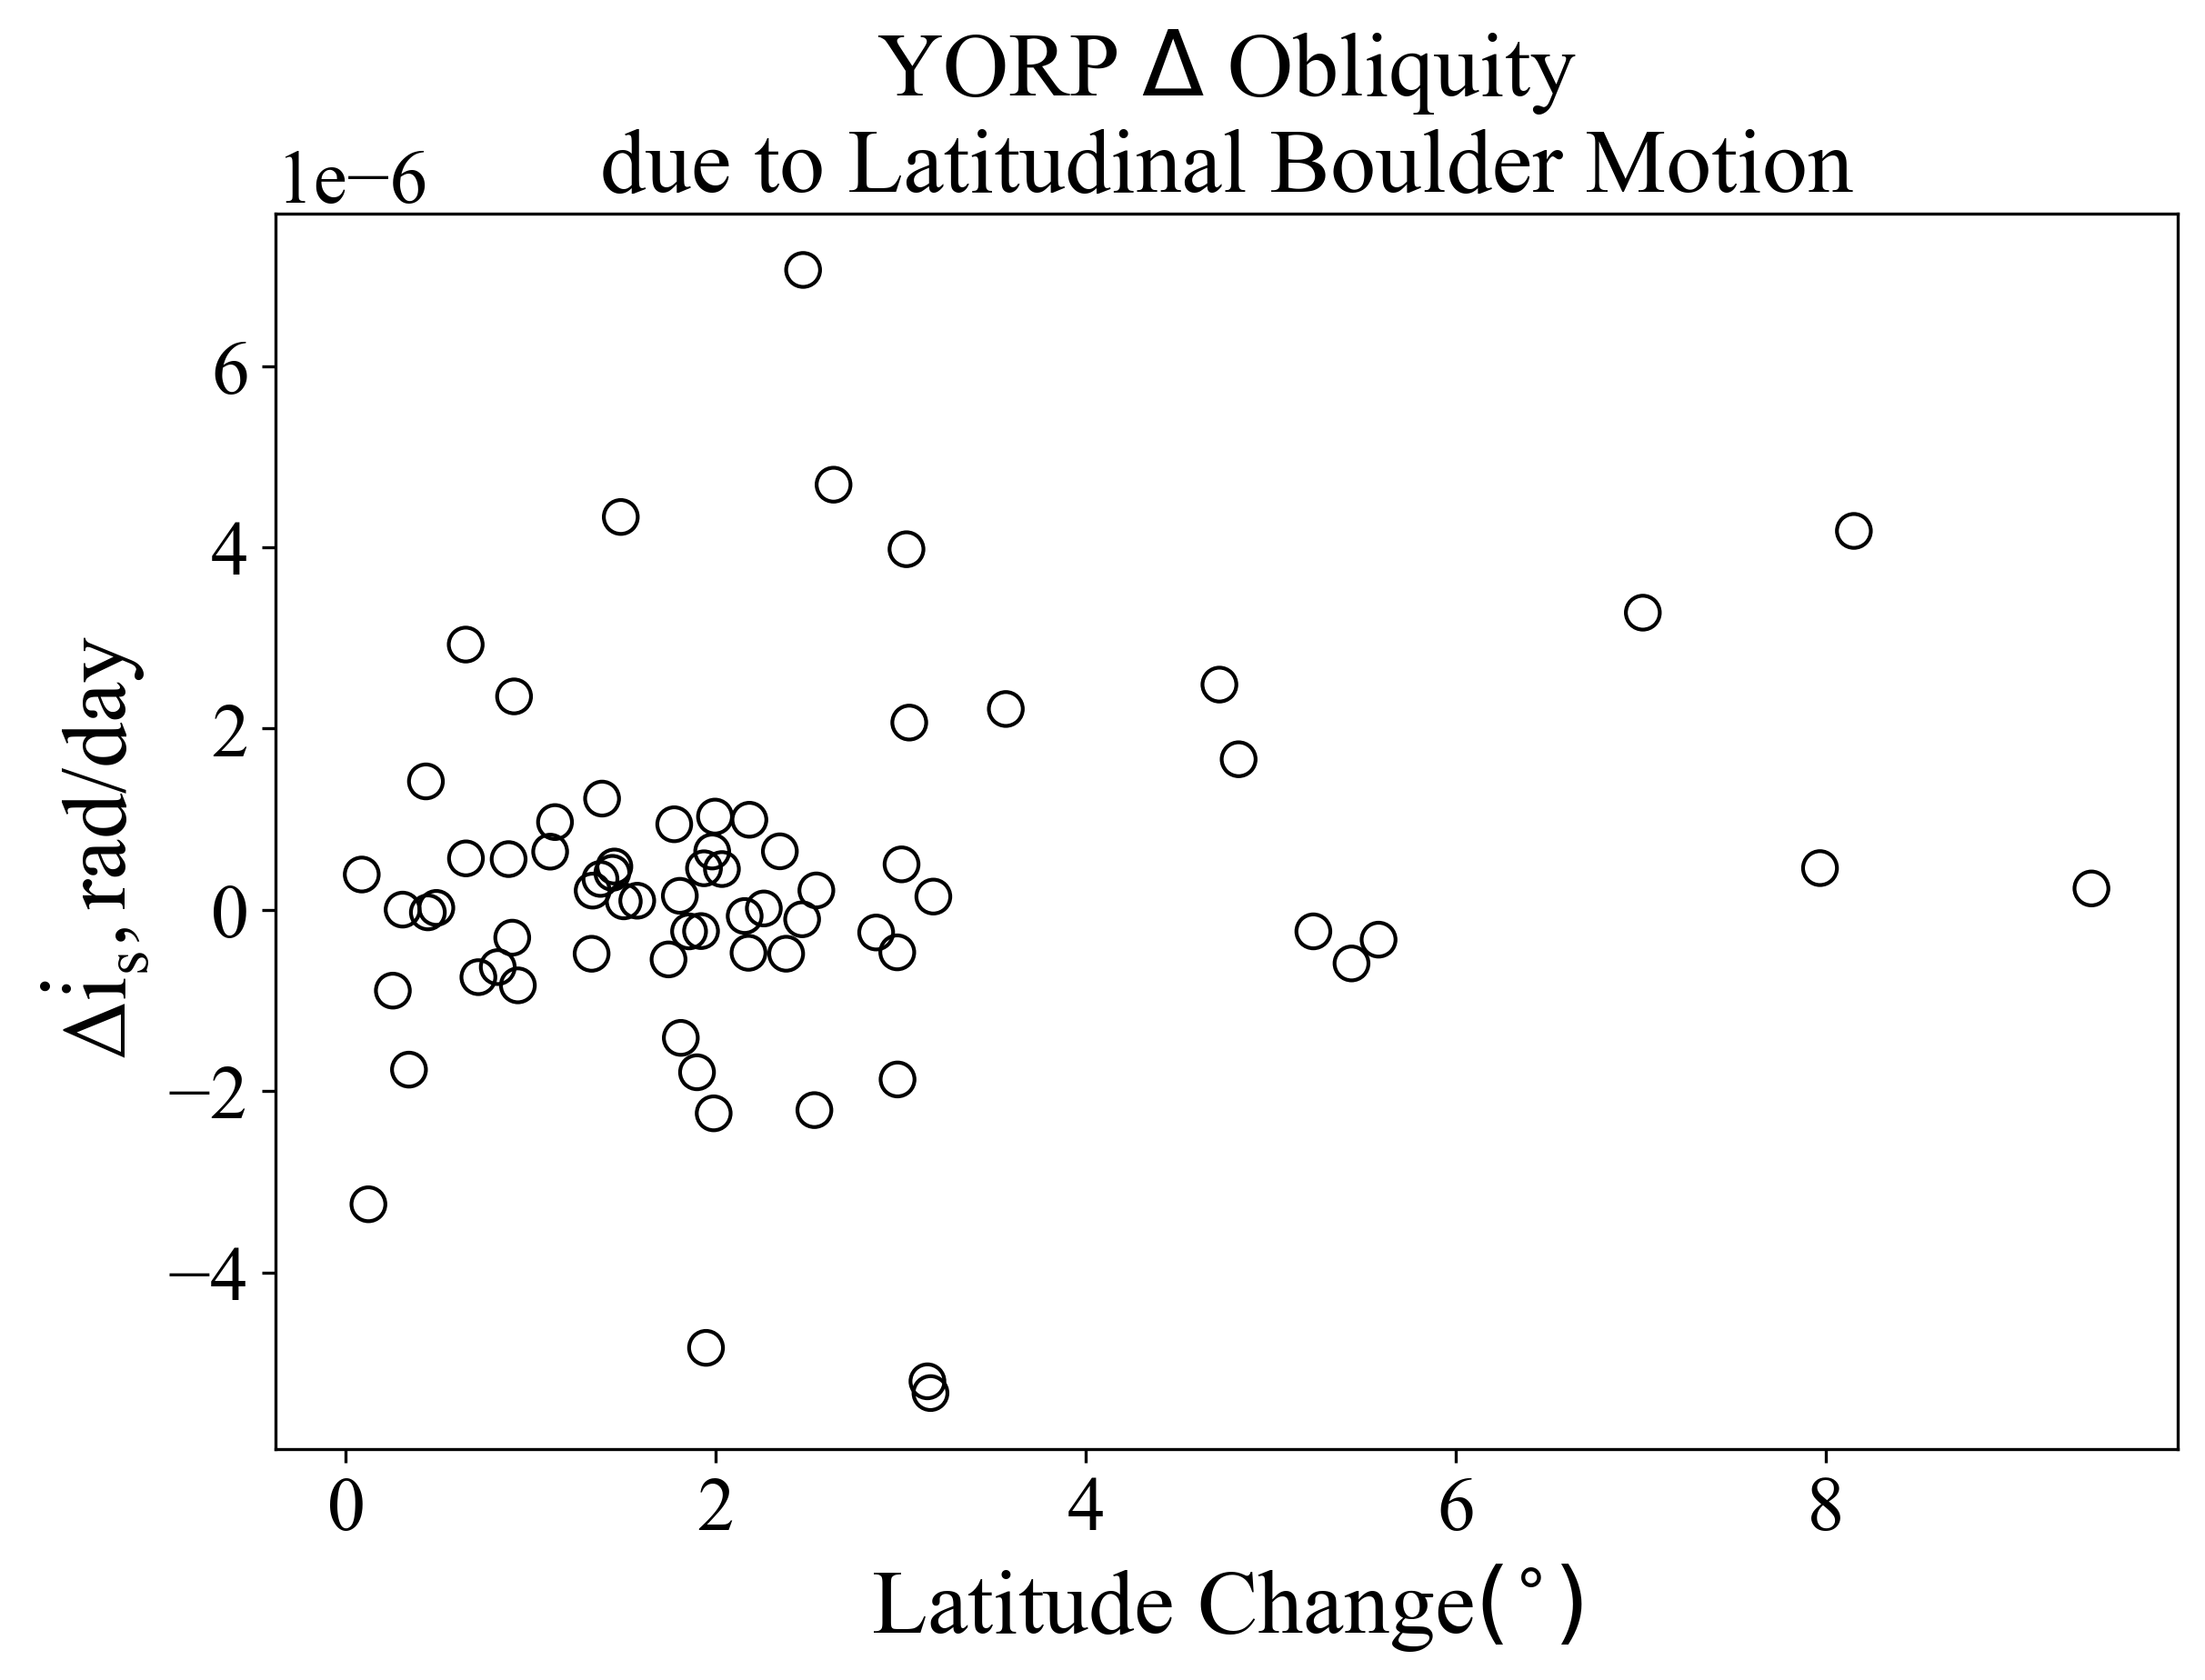
\includegraphics[width=0.5\textwidth]{fig/obliq_delta_boulder_motion_bennu.png}
    \caption{The change in YORP obliquity rate from boulder motion with the latitude degree change shown on the x-axis}
    \label{fig:ob_motion_delta}
\end{figure}


%\section{Takeaways for Obliquity Evolution} \label{conclusion}













%what did I find. Did I address the thesis I put in the intro
There are other ways of describing YORP. There are other features which induce interesting thermal effects such as self-shadowing and self-radiation (craters). Boulders move over time as the dynamics change which resets the problem. Regolith roughness can scatter the initial thermal energy and induce even more stochastics to the geometric analysis of YORP. This work has applied what we know about heavily assumed models and high-resolution asteroid surfaces to show variability in the YORP effect. Further observations of asteroid surfaces could further constrain how bouldered they get, what asymmetry is typically induced, and the thermal properties of boulders which may have been fractured, buried, or excavated as the dynamics evolve. We hope to see this continued with more advanced thermal models, the application of boulder motion based on the gravitational field variations, and rigorous ray-tracing in order to get refined YORP coefficients from the original geometries. 
